\makeatletter
\def\input@path{{../}}
\makeatother
\documentclass[../main.tex]{subfiles}
\begin{document}
\renewcommand{\path}{3_chapter_1/}
\chapter[Cyclic Peptides Permeability change based on stereocenter changes]{Modulation of the Passive Permeability of Semipeptidic Macrocycles: N- and C-Methylations Fine-Tune Conformation and Properties
    \footnote{\label{footnoteChapter5CopyRight} 
    Reprinted (adapted) with permission from Christian Comeau$^{**}$, Benjamin Ries$^{**}$, Thomas Stadelmann, and et al.,
    J. Med. Chem., \textbf{64}, 5365-5383 (2021). Copyright 2021 American Chemical Society.
    $^{**}$ equal contribution}
}
\chaptermark{Cyclic Peptides}
\label{ch:cycPep}

\aquote{``Let us learn to dream, gentlemen, and then perhaps we
shall learn the truth.''
}
{August Kekul\'e, 1865}




\begin{abstract}
Incorporating small modifications to peptidic macrocycles can have a major influence on their properties. For instance, N-methylation has been shown to impact permeability. A better understanding of the relationship between permeability and structure is of key importance as peptidic drugs are often associated with unfavorable pharmacokinetic profiles. Starting from a semipeptidic macrocycle backbone composed of a tripeptide tethered head-to-tail with an alkyl linker, we investigated two small changes: peptide-to-peptoid substitution and various methyl placements on the nonpeptidic linker. Implementing these changes in parallel, we created a collection of 36 compounds. Their permeability was then assessed in parallel artificial membrane permeability assay (PAMPA) and Caco-2 assays. Our results show a systematic improvement in permeability associated with one peptoid position in the cycle, while the influence of methyl substitution varies on a case-by-case basis. Using a combination of molecular dynamics simulations and NMR measurements, we offer hypotheses to explain such behavior.
%
\end{abstract}

\clearpage
\pagebreak

%%%%%%%%%%%%%%%%%%%%%%%%%%%%%%%%%%%%%%%%%%%%%%%%%%%%%%%%%%%%%%%%%%%%%
%% Start the main part of the manuscript here.
%%%%%%%%%%%%%%%%%%%%%%%%%%%%%%%%%%%%%%%%%%%%%%%%%%%%%%%%%%%%%%%%%%%%%
%================================================================================
\section{Introduction}
%================================================================================

Macrocycles have recently gathered increased interest in medicinal chemistry as beyond rule-of-5 (bRO5) molecules. \cite{Driggers2008, Mallinson2012, Doak2014, Dougherty2017, Marsault2011, Abdalla2018, Marsault2017, Caron2021}
A key feature of these molecules is their conformational complexity that can be leveraged in drug design to target protein-protein interactions. \cite{ Chene2006, Janin2008, Jones13, Scott2016, Modell2016}
Such protein-protein interactions are typically characterized by large flat binding sites that are difficult to target with small molecules. \cite{Doak2016}
If the macrocycles are peptidic, their toxicity is often relatively low. \cite{Zorzi2017}
Most Food and Drug Administration (FDA)-approved macrocyclic drugs belong to natural products (e.g., erythromycin, tacrolimus) or peptides (e.g., sandostatin, eptifibatide). \cite{Giordanetto2014}
Peptidic or semipeptidic scaffolds bridge the gap between small molecules and biologics. An advantage of this molecule class is that they are relatively easy to synthesis and allow a broad choice of natural and non-natural amino acids required for rapid and thorough pharmacophoric exploration. 
The main challenge with peptides resides in their physicochemical and pharmacokinetics-ADME (absorption, distribution, metabolism, and excretion) properties. 
While cyclic peptides are typically more stable to proteases compared to their linear counterparts, their high polarity often translates into low bioavailability.\cite{Naylor2017, Fosgerau2015}
However, some cyclic peptides were found to cross cell membranes.\cite{Naylor2017, Wang2014, Nielsen2014} 
Developing tools and knowledge to optimize and better predict their structure–permeability relationship is, therefore, a requirement for the field. Such quest found inspiration in studies of the cyclic undecamer cyclosporine A, which is administered orally. 
One prominent structural feature of this natural macrocycle is the high number of N-methylated residues (7 out of 11) and its dynamic structural adaptation to its environment described as chameleonic behavior. \cite{Whitty2016, Danelius2020, Witek2017}
The effect of N-methylation on the permeability of cyclic hexa- and heptapeptides has been systematically investigated since the number and position of N-methylations may be beneficial or detrimental for permeability. \cite{Nielsen2014, Raeder2018, White2011, Beck2012, Biron2008, White2011} 
%
Less explored are the N-alkylated glycines -- aka peptoids -- in which the side chain has been moved from the $\alpha$-carbon to the amide nitrogen. \cite{Schwochert2015} 
Similar to N-methylation, this modification removes one H-bond donor and removes one stereogenic center, and induces glycine-like secondary structures.
The peptoid amide also facilitates cis-trans isomerization compared to the corresponding N-methylation.\cite{Sui2007} 


More recently, the impact of the dynamics of macrocycles in response to their environment, which can range from polar in water, nonhomogeneous in the presence of its target, to lipophilic in the membrane, has been appreciated.\cite{Danelius2020, Witek2017, Riniker2019, Witek2019, Wang2021}
Studying macrocycles with computational methods leads to multiple criteria identified as being possibly essential for chameleonic behavior. Examples of these criteria are the presence of intramolecular H-bonds, 3D polar surface areas (3D-PSA), or kinetic Markov models as metrics for how macrocyclic structures yield polar atoms and rigidification of the backbone cycle into certain polar/apolar states. \cite{Witek2016, Witek2017, Tyagi2018, Witek2019, Wang2021}
A powerful tool to modulate the properties of peptidic macrocycles is the inclusion of a nonpeptidic tether unit.\cite{Marsault2007, Hoveyda2011, Roux2020} 
This tether can serve multiple purposes: in the context of a target interacting with a specific sequence, various tethers can be screened without modifying the peptide recognition sequence, while providing a simple handle for modulating affinity and pharmacokinetic properties. 
Small modifications in size, shape, or functional groups on the tether can dramatically influence on this kind of constrained system.\cite{Appavoo2019}
%
The relationship between structure and permeability is known to be elusive for this class of compounds, with small structural modifications often yielding permeability cliffs. \cite{Wang2014, Raeder2018, Beck2012, White2011, Roux2020, Bockus2015, Hewitt2015, Rezai2006, Over2016}


To investigate the structural effects of a tether with a length of five atoms and the peptide-peptoid change on the compound permeability, our collaborators synthesized a collection of 36 semipeptidic macrocycles. \cite{Comeau2021, Roux2020}
The structure of the compounds was composed of a tripeptide tethered head-to-tail with a nonpeptidic linker (Figure \ref{fig:MolDes}). 
Two classes of modifications were explored: single peptoid replacement and regio- and stereocontrolled linker C-methylation. 
%
\begin{figure}[h!]
    \centering
    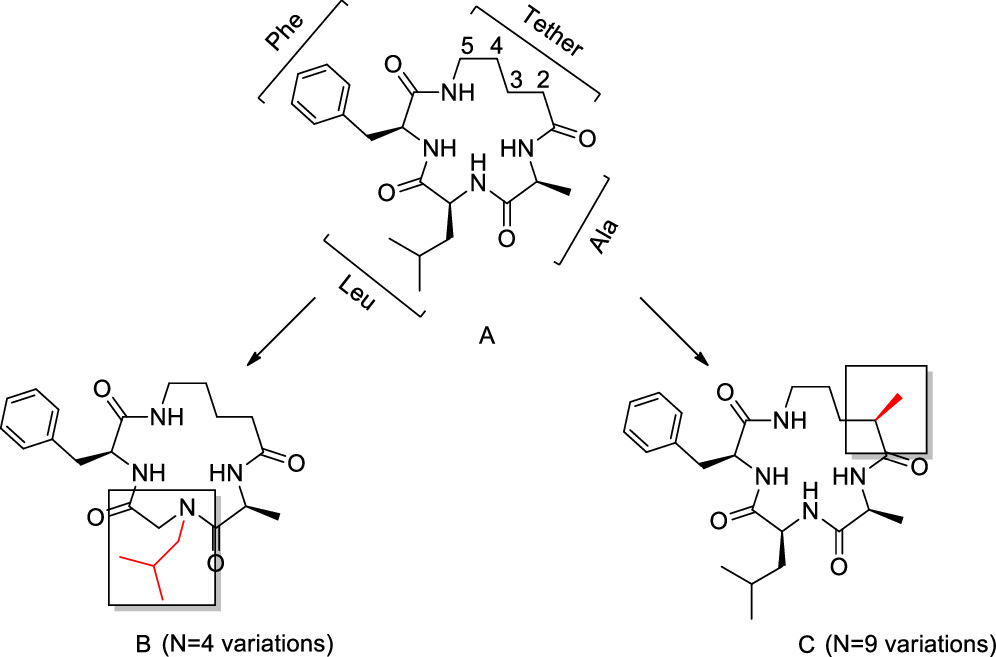
\includegraphics[width=\textwidth]{7_chapter_5/fig/intro/MoleculeDesign.jpeg}
    \caption{Synthesis strategy of our collaborators for model compound (\textbf{A}) and two types of modifications: Nala, Nleu, and Nphe peptoids (\textbf{B} showing Nleu) and regio/stereocontrolled C-methylation (\textbf{C} showing 2R methylation).\cite{Comeau2021}}
    \label{fig:MolDes}
\end{figure}

\begin{figure}[h!]
    \centering
    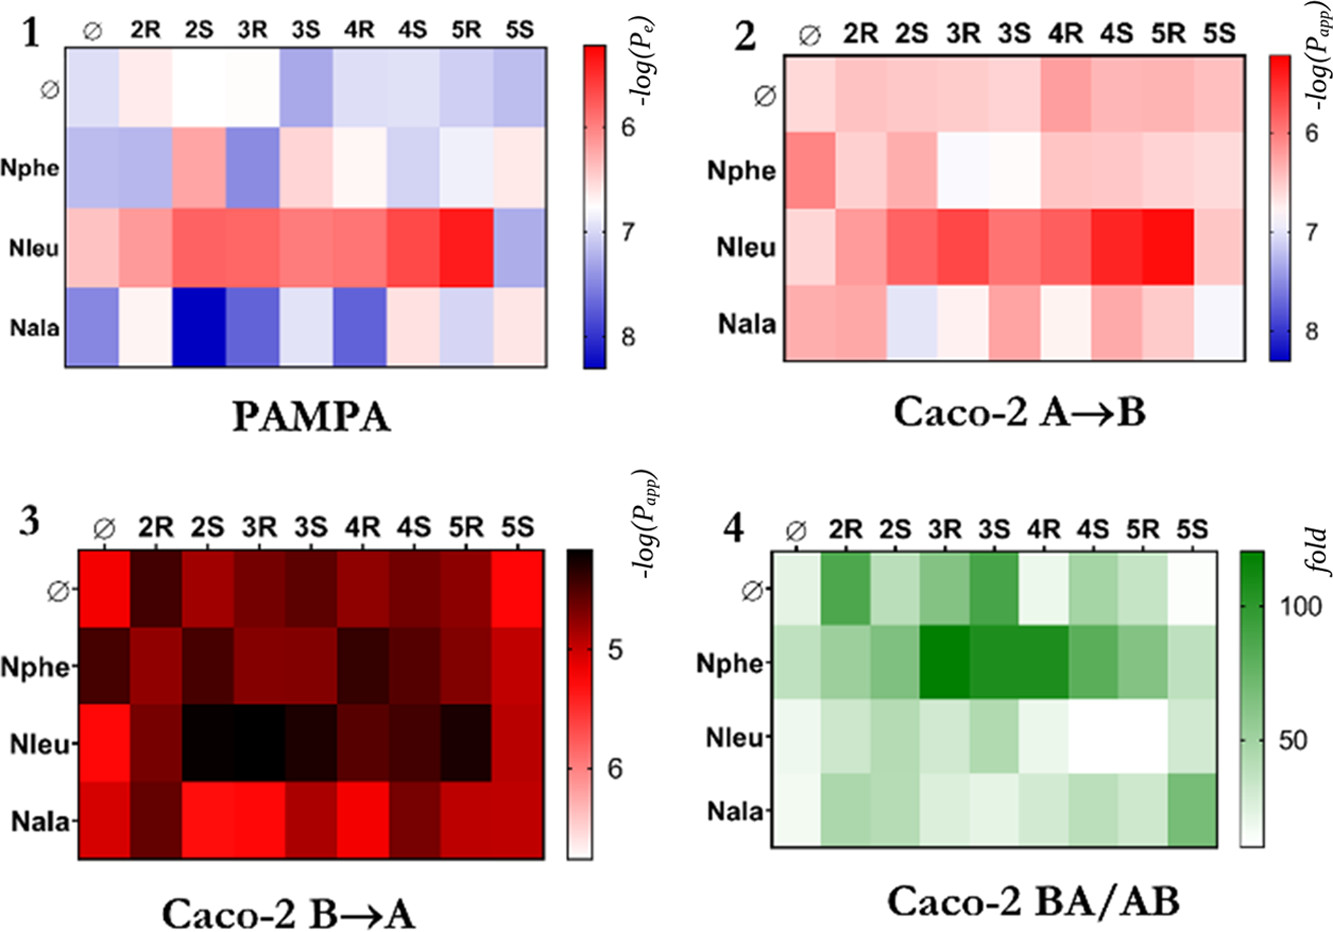
\includegraphics[width=\textwidth]{7_chapter_5/fig/intro/pampa.jpeg}
    \caption{Permeability results in the form of heatmaps. For heatmaps 1–3, the values are expressed as $−log(P_{\text{app}})$, so lower values mean higher permeability (in order of increasing permeability: blue, white, red, and black). Heatmap 4 shows the BA/AB ratio, which represents a measure of efflux.}
    \label{fig:permAssays}
\end{figure}
The passive permeability of the resulting macrocycles was measured by our collaborators in the parallel artificial membrane permeability assay (PAMPA) and their cellular permeability in the Caco-2 assay\cite{Di2015} (Figure \ref{fig:permAssays}).\cite{Comeau2021}

%
\begin{figure}
    \centering
    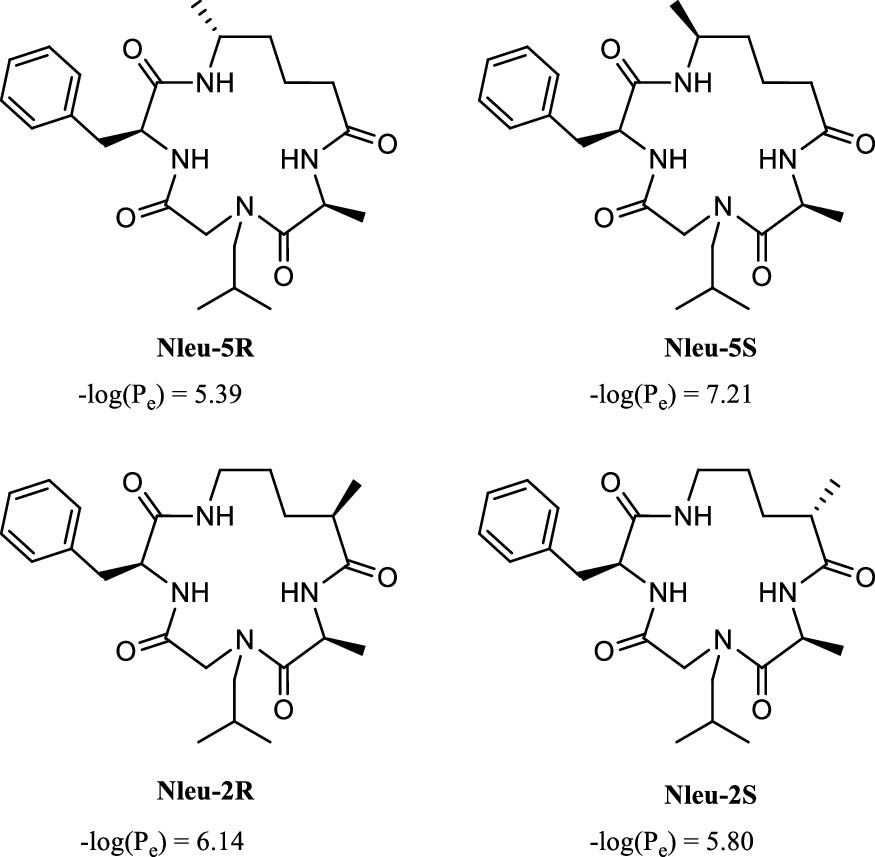
\includegraphics[width=\textwidth]{7_chapter_5/fig/intro/permCliffMols.jpeg}
    \caption{Four semipeptidic macrocycles were selected from the collection. In contrast to the pair Nleu-2R/S (bottom), the pair Nleu-5R/S (top) behave significantly  different in the permeability assays. All molecules were  studied with experimental NMR analysis and molecular dynamics (MD) simulations in a polar and apolar environment.}
    \label{fig:permCMols}
\end{figure}
Based on the permeability data, we selected two pairs of diastereomers that differ only by their stereochemistry of the tether methyl group (Figure \ref{fig:permCMols}). While one pair (Nleu-5R/S) differs greatly in their passive permeability behavior, the second one (Nleu-2R/S) does not. 
Prior studies on cyclosporine A showed that the conformational behavior of cyclic peptides in the context of membrane permeability can be studied by performing extensive molecular dynamics (MD) simulations in apolar and polar environments (e.g., chloroform and water) to mimic the behavior outside and inside a membrane. \cite{Witek2016,Witek2017, Witek2019, Wang2021}
Therefore, we carried out MD simulations of each of the four selected macrocycles in water and chloroform. The simulations results were validated by comparing to solution NMR measurements of the compounds. \cite{Balazs2019}
Finally, we used different metrics such as torsional angles, hydrogen-bond formation, and 3D-PSA\cite{Sebastiano2018} to assess and compare the conformational behavior of the compounds. 

%================================================================================
\section{Theory}
%================================================================================

%------------------------------------------------------------
\subsection{Alchemical Free-Energy Calculations}
%------------------------------------------------------------



The goal of path-dependent alchemical free-energy calculations is
to evaluate the free-energy difference $\Delta G$
between two states $A$ and $B$ of a molecular system,
by introducing a coupling scheme relying on a parameter $\lam$,
and sampling along the so-defined $\lam$-path.
%
The two states have the same number $3N$ of degrees of 
freedom, but distinct Hamiltonian functions $\ham_A(\xv)$ and $\ham_B(\xv)$,
respectively, where $\xv = (\rv,\pv)$ is the $6N$-dimensional
phase-space vector representative of a microscopic system configuration, $\rv$ 
and $\pv$ being the corresponding coordinate and momentum vectors.
%
The coupling parameter is introduced into a hybrid Hamiltonian 
$\ham(\xv;\lam)$ 
satisfying the boundary conditions
$\ham(\xv;0)=\ham_A(\xv)$ and $\ham(\xv;1)=\ham_B(\xv)$,
where the semi-colon indicates a parametric dependence.
%
%
%Examples of methods involving the coupling-parameter approach are 
%multi-configuration\cite{ST91.1} thermodynamic integration\cite{KI33.1,KI34.2,KI35.1} (MCTI or, simply, TI)
%and multi-configuration\cite{JO08.3} free-energy perturbation\cite{ZW54.1,MA95.2,LI96.1,MA99.10,SC99.3,RA12.6,RA17.5,BO17.2} (MC-FEP or, simply, FEP)
%along with their HRE\cite{SU99.1,FU02.2,ZH16.2}/HRP\cite{IT13.1,IT13.2,YA17.2} variants, as well as $\lam$-dynamics\cite{KO96.1,DA01.7,GU03.1,KN09.1,KN11.2,DO11.2,AR15.2,HA17.1} ($\lam$D),
%along with its coordinate-transformed or/and $\lam$-biased variants\cite{GU98.1,GU98.2,SO01.1,WU11.1,KN11.2,DO11.2,KN11.1,ZH12.3,DO13.1,BI14.1,BI14.2,BI15.1,BI15.2} ({\em e.g.} the $\lam$-LEUS scheme\cite{BI14.1,BI14.2,BI15.1,BI15.2}).
%
\revphildel{[-- Redundant paragraph removed --]}
%



Since the proposed CBTI scheme encompasses features of both $\lam$D and TI,
these two approaches are summarized briefly in the \radd{next two subsections.
The following three subsections then describe in turn
the basis of the CBTI scheme, 
its free-energy estimator 
and the application of a biasing potential.}



%------------------------------------------------------------
\subsection{$\lam$-Dynamics ($\lam$D)}
%------------------------------------------------------------


In the $\lam$D scheme\cite{KO96.1,DA01.7,GU03.1,KN09.1,KN11.2,DO11.2,AR15.2,HA17.1}, 
the coupling parameter $\lam$ is assigned a mass
$m_\lam$ and a momentum $p_\lam$, and considered to be an additional
pseudo-conformational degree of freedom of the system.
%
The Hamiltonian of the extended system is defined as
%
\beq{lam_dyn_ext_ham}
  \ham^\star(\xv,\lam) = \ham(\xv;\lam) + \frac{p_\lam^2}{2m_\lam} \ ,
\eeq
%
where the star refers to an extended system in which $\lambda$ 
is now a variable and no longer a parameter 
(thus the replacement of the semi-colon by a comma).
%
This leads to the additional equation of motion
%
\beq{lam_dyn_eq_mot}
  \ddot{\lam} = \frac {\dot{p}_{\lam}} {m_{\lam}} 
              = -\frac {1} {m_{\lam}} 
                 \frac {\partial\ham(\xv;\lam)} {\partial\lam}
\eeq
%
for propagating the $\lam$-variable, \radd{where a dot over a variable indicates its time derivative}.
%


The free-energy difference $\Delta G$
between the two physical end-states can then in principle be
calculated based on a single thermostated MD simulation 
of the extended system, as
%
\beq{lam_dyn_dg}
  \Delta G = 
      - \frac{1}{\beta}\ln\frac{\left\langle \delta(\lam - 1)\right\rangle^\star}
      {\left\langle \delta(\lam)\right\rangle^\star} \ ,
\end{equation}
%
where 
$\beta=(k_BT)^{-1}$, 
$k_B$ being the Boltzmann constant and $T$ the absolute temperature,
$\delta$ is the Dirac delta function, 
and $\langle\cdot\cdot\cdot\rangle^\star$ denotes ensemble averaging 
for the extended system (\ie{} over the joint trajectories of $\xv$ and $\lam$).
%
\revphil{In practice, the $\delta$-functions in \refeq{lam_dyn_dg} must be replaced
      by two finite end-state bins ($\lambda$-cutoff), sufficiently large
      for proper statistics but also sufficiently small for avoiding 
      distortions due to averaging at the end-states\cite{KN11.1}.}
%
\revphildel{[-- Redundant paragraph removed --]}
%
%There are, however, a number of important practical issues 
%to be addressed if this scheme is to be accurate and efficient\cite{BI14.1}:
%%
%($i$) the variations of $\lam$ must be restricted to the range $[0,1]$ between the two physical end-states\cite{KO96.1};
%($ii$) the mass and thermostat-coupling scheme of the $\lam$-variable must be chosen appropriately
%      to ensure a correct temperature for this variable\cite{BI15.1};
%($iii$) the sampling along $\lam$ must generally be adjusted
%      to ensure adequate sampling of the A and B states
%      with a sufficient number of interconversion transitions\cite{BI14.1};
%($iv$) the $\delta$-functions in \refeq{lam_dyn_dg} must be replaced
%      by two finite end-state bins ($\lambda$-cutoff), sufficiently large
%      for proper statistics but also sufficiently small for avoiding 
%      averaging distortions at the end-states\cite{KN11.1}. %
%%
%Different implementation variants of $\lambda$D address these
%issues in a variety of ways, including the use of
%coordinate transformations\cite{KN11.2,DO11.2,WU11.1,KN11.1,DO13.1,ZH12.3,BI14.1,BI15.2},
%memory-based biasing potentials,\cite{GU98.1,GU98.2,SO01.1,WU11.1,BI14.1,BI15.2}
%separate thermostat coupling of the $\lam$-variable\cite{BI14.1,BI15.1,BI15.2},
%and 
%alternative free-energy estimators\cite{LU04.3,SH05.6,KA05.1,KA06.6,FA09.4,KA12.5,TA12.1,DI17.5,ZH17.6}.



%------------------------------------------------------------
\subsection{Thermodynamic Integration (TI)}
%------------------------------------------------------------


In the original TI scheme\cite{KI33.1,KI34.2,KI35.1}, a set of 
$K$ replicas of the system are simulated in parallel at fixed predefined 
$\lam$-values in the range $[0,1]$.
Since the replicas are entirely decoupled 
from each other, the simulations
can be performed serially as well. However, TI extensions 
including the HRE scheme\cite{SU99.1,FU02.2,ZH16.2} and the HRP scheme\cite{IT13.1,IT13.2,YA17.2}
introduce a coupling in the form of $\lam$-value exchanges,
in which case the simulations must really be carried out in parallel.
The same will apply to the proposed CBTI scheme, where the coupling involves a synchronization of
the dynamical $\lam$-variations. 


Considering all replicas $k=0 \dots K-1$ as the members of a replica system,
one may note the corresponding $6K\mkern-3mu\times\mkern-3mu N$-dimensional phase-space vector
as $\Xv=\{\xv_k\}$ and the corresponding $K$-dimensional vector containing the fixed $\lam$-values as 
$\lamv=\{\lam_k\}$.
%
In plain TI, the Hamiltonian of the replica system is defined as
%
\beq{ti_rep_ham}
  \ham^\dagger(\Xv;\lamv) = \sum_{k=0}^{K-1} \ham(\xv_k;\lam_k) \ ,
\eeq
%
where the dagger refers to a replica system,
and $\lamv$ is here a parameter vector (thus the semi-colon).
Because the Hamiltonian of \refeq{ti_rep_ham} involves no coupling 
term  between the replicas, the dynamics of a replica $k$
is independent from that of the other replicas and
solely depends on $\lam_k$.


The free energy difference $\Delta G$
between the two states can then be
calculated based on a single thermostated MD simulation 
of the replica system, as
%
\begin{multline}
  \label{eq:ti_formula}
  \Delta G = 
  \int\limits_0^1 \mathrm{d}\lam' \left\langle \frac{\partial{\ham(\xv;\lam)}}{\partial \lam} \right\rangle_{\lam'} 
    \approx
    \sum_{k=0}^{K-1}  w_k \left\langle \frac{\partial{\ham^\dagger(\Xv;\lamv)}}{\partial \lam_k} \right\rangle^\dagger\\ 
    = 
    \sum_{k=0}^{K-1}  w_k \left\langle \frac{\partial{\ham(\xv_k;\lam_k)}}{\partial \lam_k} \right\rangle^\dagger \ ,
\end{multline}
%
where 
the $w_k$ are quadrature weights for the numerical integration\cite{JO10.2,BR11.5,BR11.6},
$\langle\cdot\cdot\cdot\rangle_{\lam}$ denotes ensemble averaging 
for a single system \radd{(\ie{} over $\xv$) at the given $\lam$ value},
and
$\langle\cdot\cdot\cdot\rangle^\dagger$ denotes ensemble averaging 
for the replica system (\ie{} over $\Xv$).


\revphil{In the above form, TI has long been the workhorse of alchemical free-energy calculations.
%
The method is extremely robust in the sense 
that the accuracy of the calculated $\Delta G$
%free-energy change 
can always be systematically
improved (more $\lambda$-points, longer equilibration or/and sampling times).
However, it is not necessarily the most 
%practical and 
efficient 
method to determine $\Delta G$ up to a certain accuracy,
due to possible sub-optimalities in
the coupling scheme\cite{CR86.1,BL04.2,PH11.1,PH12.1,NA14.1,NA15.3},
the protocol design\cite{ME93.3,HU16.7,ME17.1,SU17.3,DA18.1}
the free-energy estimator\cite{LU04.3,SH05.6,SH08.7,FA09.4,TA12.1,DE16.9,DI17.5,ZH17.6},
and
the orthogonal sampling\cite{WO03.1,WO03.2,KH10.1,KH11.2,BI15.1}.
}
\revphildel{[-- Redundant paragraph removed --]}




%In the above form, TI has long been the workhorse 
%of alchemical free-energy calculations.
%%
%In practice, in addition to the choice of a coupling scheme\cite{CR86.1,BL04.2,PH11.1,PH12.1,NA14.1,NA15.3},
%a TI calculation requires the definition of a protocol including:
%($i$) the number $K$ and distribution (spacing) of the $\lambda$-points considered;
%($ii$) the initial configurations, equilibration times and sampling times
%    selected for each $\lambda$-point;
%($iii$) the choice of a quadrature scheme for the numerical integration.
%%
%The accuracy of the calculation will depend on the selection of these 
%parameters, the optimization of which may represent a non-trivial and 
%time-consuming task\cite{ME93.3,HU16.7,ME17.1,SU17.3,DA18.1}.
%%
%Thus, even though TI is extremely robust in the sense 
%that the accuracy of the calculated free-energy change can always be systematically
%improved (more $\lambda$-points, longer equilibration or/and sampling times),
%it is not necessarily the most efficient method to determine 
%$\Delta G$ up to a certain accuracy.
%
%Many improvements have been proposed for the TI scheme
%over the years.
%%
%Most prominently, the inclusion of $\lam$-exchanges in 
%%HRE\cite{SU99.1,FU02.2,ZH16.2}/HRP\cite{IT13.1,IT13.2,YA17.2} 
%\radd{the HRE scheme\cite{SU99.1,FU02.2,ZH16.2} and the HRP scheme\cite{IT13.1,IT13.2,YA17.2}}
%permits to 
%circumvent orthogonal barriers\cite{WO03.1,WO03.2,KH10.1,KH11.2}, a feature also shared by $\lambda$D schemes\cite{BI15.1}, and
%the use of alternative free-energy estimators like the
%EXTI\cite{DE16.9} scheme or the MBAR\cite{SH08.7} scheme permits to improve the statistical efficiency.



%------------------------------------------------------------
\subsection{Conveyor Belt Thermodynamic Integration (CBTI)}
%------------------------------------------------------------


The proposed CBTI scheme encompasses features of both $\lam$D and TI.
%
Similarly to TI, it is based on the simulation of a replica system involving 
$K$ copies of the molecular system of interest, where $K$ is taken to be even.
%
And similarly to $\lam$D, the individual replicas are extended 
systems, for which the associated $\lam_k$-variable is allowed to evolve
along the simulation.
%
However, the evolutions of these $\lam_k$-variables are not independent. 
They are coupled to each 
other by means of a sequence of hard constraints,
 so that they follow the course of a conveyor belt (CB).
Thus, they are entirely determined by a single dynamical
variable $\Lamb$, following 
the scenario depicted in \reffig{scheme} and discussed
in the Introduction section.



The variable $\Lamb$ is a continuous real variable
representing the overall advance of the CB, successive multiples
of $2\pi$ corresponding to as many full rotations.
%
%
Given $\Lamb$ and $K$, the $\lam$-value $\lam_k$ associated with a system $k$ on the CB
is obtained as
%
\beq{cb_lam_of_big_lam}
  \lam_k(\Lamb) = \zeta\left( \Lamb + k \Delta\Lamb  \right) \ ,
\eeq
%
\radd{with
\beq{delta_lamb}
\Delta\Lamb = 2\pi K^{-1} .
\eeq
}
\radd{Here, the function $\zeta$} is a continuous and periodic zig-zag function of period $2\pi$ and image range $[0,1]$,
defined over the reference period $[0,2\pi)$ as
%
\beq{zigzag_fct}
  \zeta(\theta) = \left\{
                    \begin{array}{ll}
                       \pi^{-1}\theta & \mathrm{if}\ \theta < \pi \\
                       2-\pi^{-1}\theta & \mathrm{if}\ \theta \geq \pi \\
                    \end{array} 
                  \right. \ \ \mathrm{for}\ \theta\in[0,2\pi) \ ,
\eeq
%
where the $[\cdot,\cdot)$ indicates an interval that is open to the right side, {\em e.g.} $[0,2\pi)$ includes $0$ but excludes $2\pi$.
%
\radd{An advance of the CB by $\Delta\Lamb$}
%
corresponds to a cyclic permutation of the $K$ replicas, each system moving by 
one position forward along the CB, \ie
$\lam_k(\Lamb+\Delta\Lamb) = \lam_{k+1}(\Lamb)$
for $k<K-1$, along with
$\lam_{K-1}(\Lamb+\Delta\Lamb) = \lam_0(\Lamb)$.
%
For this reason, the increment $\Delta \Lamb$ will be further referred to 
as one shift of the CB.
%
The system $k=0$ can be viewed as a reference system,
as $\lambda_0=\pi^{-1}\Lambda$ for $0\leq\Lambda<\pi$
and $\lambda_0=2-\pi^{-1}\Lambda$ for $\pi\leq\Lambda<2\pi$.
%
Since $K$ is chosen to be even, an increase of $\Lambda$
always corresponds to an increase of $\lambda_k$
for half of the systems (forward-moving side of the CB)
and a decrease of $\lam_k$ for the other half of the systems
(backward-moving side of the CB). This choice also implies that 
$\Lamb$-values which are integer multiples of the
CB shift $\Delta \Lamb$ 
correspond to situations where there is 
one system in state $A$ and one system in state $B$.
%
Since an advance of the CB variable by $2\pi$
leaves the replica system invariant, 
the variable $\Lamb$ will commonly be refolded into the 
reference period $[0,2\pi)$ when illustrating the
results of the CBTI method.

The Hamiltonian of the extended replica system is defined as
%
\beq{cb_ext_rep_ham}
  \ham^{\dagger\star}(\Xv,\Lamb) = \ham^\dagger(\Xv;\lamv)  +  \frac{p_\Lamb^2}{2m_\Lamb} 
  \quad \text{with} \quad \lamv=\lamv(\Lamb),
\eeq
%
%
where $\ham^{\dagger}$ is defined as in TI by \refeq{ti_rep_ham}
and $\lamv(\Lamb)$ by \refeq{cb_lam_of_big_lam}.
%
In analogy with \refeq{lam_dyn_eq_mot}, the resulting equation of motion for $\Lamb$ reads
%
\beq{cb_big_lam_eq_mot}
  \ddot{\Lamb} = \frac {\dot{p}_{\Lamb}} {m_{\Lamb}} 
              = -\frac {1} {m_{\Lamb}}  \frac {\partial\ham^\dagger(\Xv;\lamv)} {\partial \Lamb} 
\eeq
%
where
%
\begin{align}
  \label{eq:cb_big_lam_eq_mot_der}
   \frac{\partial\ham^\dagger(\Xv;\lamv)}{\partial\Lamb}
        &= \sum_{k=0}^{K-1} \frac {\partial\ham(\xv_k;\lam_k)} {\partial \lam_k} \frac{\mathrm{d} \lam_k}{\mathrm{d} \Lamb}\nonumber \\
        &= \sum_{k=0}^{K-1} \frac {\partial\ham(\xv_k;\lam_k)} {\partial \lam_k} \zeta'\left( \Lamb + 2\pi K^{-1} k \right) \ .
\end{align}
%
Here, the function $\zeta'$ is the derivative of the zig-zag function of \refeq{zigzag_fct}, 
given over the reference period $[0,2\pi)$ by
%
\beq{zigzag_der}
  \zeta'(\theta) = \left\{
                    \begin{array}{ll}
                       \pi^{-1} & \mathrm{if}\ \theta < \pi \\
                       -\pi^{-1} & \mathrm{if}\ \theta \geq \pi \\
                    \end{array} 
                  \right. \ \ \mathrm{for}\ \theta\in[0,2\pi) \ .
\eeq
%
Formally, the derivative is not defined when $\theta$
is an integer multiple of $\pi$, \ie{} for a system that is exactly 
in one of the physical end-states $A$ or $B$. In this case, the value of $\zeta'$ has been arbitrarily set to 
$\pi^{-1}$ for even multiples and $-\pi^{-1}$ for odd multiples.
This has a negligible impact in practice, as it only concerns a series
of infinitesimal points over the entire $\Lamb$-range, 
\ie{} infinitesimally few configurations along a CBTI simulation.
%
\revphil{For example, when using double-precision floating-point arithmetics
(including denormalized numbers),
their probability of occurrence is on the order of 10$^{-324}K$ 
({\em i.e.} a single expected occurrence over a simulation lasting about 10$^{292}K^{-1}$
times the age of the universe with a 2 fs timestep).
}
%
Neither does going over the discontinuity within a timestep represent a source of non-conservativeness. The concerned replica
will merely bounce back the corresponding physical end-state with a reversion of its velocity, akin to a particle reflected elastically
by a hard wall (delta-function force).
%
If desired, these \revphil{exceptional points could be handled
more formally by altering} the definition of $\zeta$,
\revphil{{\em e.g.} by smoothing its tips in a narrow range around $0$ and $\pi$}.


The $\lam_k$-dynamics of the individual systems is entirely
specified by \refeq{cb_big_lam_eq_mot} to propagate $\Lamb$
along with  \refeq{cb_lam_of_big_lam} to calculate the $\lam_k$-values from the current $\Lamb$.
Alternatively, one may write an equation of motion for the $\lambda_k$-variables of the 
individual replicas by combining the two equations (along with \refeq{cb_big_lam_eq_mot_der}) as
%
\begin{align}
  \label{eq:cb_lam_eq_mot}
  \ddot{\lam}_k &= \ddot{\Lamb} \frac{\mathrm{d} \lam_k}{\mathrm{d} \Lamb} + \dot{\Lamb}^2 \frac{\mathrm{d^2} \lam_k}{\mathrm{d} \Lamb^2} \nonumber\\
                &= -\frac {1} {m_{\Lamb}} \left( 
                       \sum_{l=0}^{K-1} \frac {\partial\ham(\xv_{l};\lam_{l})} {\partial \lam_{l}} \zeta'\left( \Lamb + 2\pi K^{-1} l \right) 
                       \right) \nonumber  \\
                   & \qquad \zeta'\left( \Lamb + 2\pi K^{-1} k \right) \ .
\end{align}
%
%
Note that the term in $\dot{\Lamb}^2$ vanishes since the second derivative $\zeta''$ of $\zeta$
is zero (except at the \radd{exceptional} singular points). However, it should not be overlooked 
if one decides to use a different function $\zeta$.
%
Introducing the vector $\Dv$ and the symmetric $\Lamb$-dependent matrix $\Cmat$ defined 
by their components as
%
\begin{multline}
  \label{eq:cb_def}
 D_k = \frac{\partial\ham(\xv_{k};\lam_{k})}{\partial \lam_{k}}
\ \ \ \mathrm{and}\\
C_{kl}(\Lambda) = \pi^2 \zeta'\left( \Lamb + 2\pi K^{-1} k \right) \zeta'\left( \Lamb + 2\pi K^{-1} l \right) \ ,
\end{multline}
%
\refeq{cb_lam_eq_mot} can be rewritten in an elegant matrix form as
%
\beq{cb_lam_eq_mot_mat}
  \ddot{\lamv} = -\frac {\Cmat(\Lamb)} {\pi^2 m_{\Lamb}}  \Dv \ .
\eeq
%
The elements of the symmetric matrix $\Cmat$
are either -1 (pair of systems currently on opposite sides of the CB,
and thus moving in opposite directions) or +1
(pair of systems currently on the same side of the CB, and thus moving in the same direction). The diagonal elements
are all +1, and the other +1 values surround the diagonal (line- and column-wise),
the rest being -1 values.
Because $K$ is even, the two types of values 
are always equally represented in the matrix, 
specific locations
depending on $\Lamb$.
%
Note that the variable $\Lamb$ itself still needs to be explicitly propagated
using \refeq{cb_big_lam_eq_mot}.

%%\revphil{Discussion in page 16-18 a little hard to get through.}

For a given configuration $\Xv$ of the replica system, the Hamiltonian
$\ham^\dagger$ of \refeq{ti_rep_ham} (together with \refeq{cb_lam_of_big_lam}) is periodic in $\Lamb$ 
with a period $2\pi$ corresponding to a full rotation of the CB.
%
However, because the Hamiltonians of the individual replicas are 
identical, upon ensemble averaging over $\Xv$, 
one expects the calculated properties to be periodic over $\Lamb$ 
with a smaller period $\Delta \Lamb$, corresponding to one shift of the CB.
%
\revphil{
This is in particular the case for the probability distribution $P(\Lamb)$
along $\Lamb$ and the associated free-energy profile $G_{\Lamb}(\Lamb)$,
given by
%
%\begin{align}
%\label{eq:fre_prof_lam_def}
%%\beq{fre_prof_lam_def}
%  G_{\Lamb}(\Lamb) &= G_{\Lamb}(0) +
%      \int\limits_0^\Lamb \mathrm{d}\Lamb' \left\langle \frac{\partial{\ham^{\dagger}(\Xv;\lamv)}}{\partial \Lamb} \right\rangle^{\dagger}_{\Lamb'} \\ \nonumber
%    &=  G_{\Lamb}(0) + \sum_{k=0}^{K-1}  \left[ G(\lam_k(\Lamb)) - G(\lam_k(0))\right] \quad \text{with} \  \lamv=\lamv(\Lamb) \ ,
%\end{align}
%
\begin{align}
  \label{eq:fre_prof_lam_def}
  G_{\Lamb}(\Lamb) &= G_{\Lamb}(0) +
      \int\limits_0^\Lamb \mathrm{d}\Lamb' \left\langle \frac{\partial{\ham^{\dagger}(\Xv;\lamv)}}{\partial \Lamb} \right\rangle^{\dagger}_{\Lamb'} \nonumber \\
    &=  \tilde{G}_{\Lamb}(0) + \sum_{k=0}^{K-1} G(\lam_k) \quad \text{with} \  \lamv=\lamv(\Lamb) \ ,
\end{align}
%
where $\lamv(\Lamb)$ is defined by \refeq{cb_lam_of_big_lam},
$\langle\cdot\cdot\cdot\rangle^{\dagger}_{\Lamb}$ denotes ensemble averaging 
for the replica system (\ie{} over $\Xv$) at the given $\Lamb$ value,
and the second equality follows from \refeqs{ti_rep_ham} and \refeqn{ti_formula}
(the unknown constant $\tilde{G}_{\Lamb}(0)$ 
is equal to $G_{\Lamb}(0)$ increased by a sum of $-G(\lam_k(0))$
offsets).
%
}
%


\radd{Owing to this periodicity over a smaller interval}, it is convenient to introduce a fractional advance variable $\tilde{\Lamb}$
defined as
%
\beq{tilde_lamb_def}
   \tilde{\Lamb} = \gamma( \Lamb, \Delta \Lamb ),
\eeq
%
where
%
\beq{gamma_def}
   \gamma(\theta,\theta_o)
     = \theta_o  \left( \theta_o^{-1}\theta - \lfloor \theta_o^{-1}\theta \rfloor \right)
\eeq
%
returns the part of $\theta$ in excess of the closest lower integer multiple of $\theta_o$.
%
In contrast to $\Lamb$, which is an unbounded variable, $\tilde{\Lamb}$ only spans a finite definition interval $[0,\Delta \Lamb)$.
%
At full convergence, 
any average property binned as a function 
of $\Lambda$ over the interval $[0,2\pi)$ will 
consist of $K$ successive repeats of the same property binned
as a function of $\tilde{\Lambda}$ over its definition interval $[0,\Delta \Lamb)$, as observed in \reffig{scheme:ene:sinus} for the free energy \radd{$G_{\Lamb}(\Lamb)$}.
%
Accordingly, in the absence of full convergence
along $\Lambda$, binning as a function of $\tilde{\Lambda}$
over the interval $[0,\Delta \Lamb)$ followed by $K$-fold replication
provides an efficient way to construct a more accurate representation of any 
$\Lambda$-resolved average quantity. In fact, the definition interval of $\tilde{\Lamb}$ could be further halved by noting that, upon ensemble averaging over $\Xv$ and for any $\Lamb$ value that is an integer multiple of $\Delta \Lamb$, a forward move of the CB produces the same result as a backward move of the same magnitude. Consequently, $\Lamb$-resolved average properties are even over successive $2\pi K^{-1}$ intervals, as also observed in \reffig{scheme:ene:sinus} for the free energy
\radd{$G_{\Lamb}(\Lamb)$}. The corresponding information is thus entirely encompassed in an interval of size $\Delta \Lamb /2$.

The normalized probability distribution $p(\lam)$ 
along the coupling variable $\lam$ considering all the replicas is defined by
%
\beq{proba_of_lam}
  p(\lam) = K^{-1} \sum_{k=0}^{K-1} \left\langle \delta(\lam_k-\lam) \right\rangle^{\dagger\star} \ ,
\eeq
%
\radd{where $\langle\cdot\cdot\cdot\rangle^{\dagger\star}$ denotes ensemble averaging 
for the extended replica system (\ie{} over the joint trajectories of $\Xv$ and $\lamv$).}
%
At full convergence, this probability over the interval $[0,1]$
will consist of $K/2$ successive
repeats of the corresponding distribution over the interval $[0,2 K^{-1})$.
%
\radd{More precisely, the distribution $p(\lam)$} is related to the distribution 
$\tilde{P}(\tilde{\Lamb})$ of $\tilde{\Lamb}$ over interval $[0,\Delta \Lamb)$
as
%
%\revdavid{Shouldn't there be a factor, \ie
\beq{proba_of_lam_from_that_of_big_lam}
%  p(\lam) = \tilde{P}( \pi \gamma( \lam, 2 K^{-1} )  ) \ .
  p(\lam) = \Delta \Lamb\,\tilde{P}( \pi \gamma( \lam, \pi^{-1}\Delta\Lamb )  )  \ .
\eeq
%}
%
%\beq{proba_of_lam_from_that_of_big_lam}
%%  p(\lam) = \tilde{P}( \pi \gamma( \lam, 2 K^{-1} )  ) \ .
%  p(\lam) = \tilde{P}( \pi \gamma( \lam, \pi^{-1}\Delta\Lamb )  ) \ .
%\eeq
%
In plain words, this means that $\tilde{P}(\tilde{\Lamb})$ is the relevant quantity
in terms of sampling along the coupling variable $\lam$.
If it is close to uniform over the range $[0,\Delta \Lamb)$,
then $p(\lam)$ will also be close to uniform over the range $[0,1]$.
Here again, it is noted that $p(\lam)$ is also even over the interval $[0,2 K^{-1})$,
and could be mapped to a $\tilde{\Lamb}$ value defined over an interval of size $\Delta \Lamb / 2$ instead of $\Delta \Lamb$ if desired, as

\beq{sym_proba_lam}
  p(\lam) = \left\{
                    \begin{array}{ll}
%                       \tilde{P}(\pi \gamma(\lam, 2 K^{-1})) & \mathrm{if}\ \gamma(\lam, 2 K^{-1}) < K^{-1} \\
                       \Delta \Lamb\,\tilde{P}(\pi \gamma(\lam, \pi^{-1}\Delta\Lamb)) & \mathrm{if}\ \gamma(\lam, \pi^{-1}\Delta\Lamb) < (2\pi)^{-1}\Delta\Lamb \\
%                       \tilde{P}(\pi \gamma(1-\lam,  2 K^{-1})) & \mathrm{otherwise} \\
                       \Delta \Lamb\,\tilde{P}(\pi \gamma(1-\lam,  \pi^{-1}\Delta\Lamb)) & \mathrm{otherwise} \\
                    \end{array} 
                  \right. .
\eeq


\radd{
%------------------------------------------------------
\subsection{CBTI Free-energy Estimator}
%------------------------------------------------------------
}


Due to the constraints coupling the $\lam_k$-values of the
$K$ replicas, the function $p(\lam)$ of \refeq{proba_of_lam}
is by no means a Boltzmann distribution in terms of the single-system
Hamiltonian. In fact, as seen above, it consists at full convergence
of $K/2$ successive repeats of the same even
curve.
In addition, compared to the Boltzmann distribution,
it will be
significantly flatter. On the one hand, the smaller amplitude of variations 
%and the reduced barriers 
are desired, as they will lead to more homogeneous sampling 
and \revphil{are expected to ease transitions along $\Lamb$ 
(up to the limit imposed by the speed of random diffusion)}.
%
%\revphil{
%Page 18: says that 'there is a smaller amplitude of variations and
%reduced barriers', but it's not clear dynamics are faster, since the
%dH/dl force is slowed down by (averaged). I think this is eventually
%explained by the fact that it becomes nearly diffusive behavior, but
%perhaps this can be brought up sooner.
%}
%
%
On the other hand, it is no longer possible to evaluate 
the free-energy difference $\Delta G$
directly from $p(\lam)$ in analogy with the $\lam$D expression of \refeq{lam_dyn_dg}.
%
However, since the dynamics remains Hamiltonian and the coupling 
between replicas does not
involve the configurational degrees of freedom, the change \radd{from TI to CBTI} does not affect 
the conditional probabilities $\mathcal{P}(\xv | \lam)$. Thus,
configurational ensemble averages sorted by $\lam$-values will remain
identical to those one would obtain from TI \radd{(or from HRE/HRP or $\lam$D)}.
%
As a result, $\Delta G$ can still be obtained 
\radd{by integrating over the average Hamiltonian derivative binned as a function 
of $\lambda$ considering all replicas simultaneously,}
in analogy with the TI expression
of \refeq{ti_formula}.
%
\revphil{Note that the exceptional points of the function $\zeta'$
(discussed previously in the context of \refeq{zigzag_der})
have no influence on the integration, as they represent
finite discontinuities over infinitesimal ranges.
}
%\revphil{SAY THAT DISCONT HAS NO EFFECT
%See Point 6 above. Similar considerations apply to the integration.
%We integrate $\partial\mathcal{H}/\partial\lam$. If the value is off
%at one (or a few) points, the integral is unaffected because the 
%neighborhood of the singularity is infinitesimal and its magnitude
%is finite ({\em i.e.} it is not a $\delta$ function, but just 
%a finite change in the function value).
%}



In practice, \revphil{$\Delta G$} is calculated here based on a single thermostated MD simulation 
of the extended replica system, as
%
\begin{align}
\label{eq:cbti_formula}
  \Delta G &= 
    \int_0^1 \mathrm{d}\lam' K^{-1} \sum_{k=0}^{K-1} \left\langle 
                 \frac{\ham(x_k;\lam_k)}{\partial \lam_k} \delta(\lam_k-\lam')
            \right\rangle^{\dagger\star}\\ \nonumber
   &\approx
%     K^{-1} 
\sum_{j=0}^{J-1}  \left \langle \frac{ \sum_{k=0}^{K-1} \frac{\ham(x_k;\lam_k)}{\partial \lam_k} \alpha(\lambda_k,j;J)}
                              { \sum_{k=0}^{K-1} \alpha(\lambda_k,j;J)}  \right \rangle^{\dagger \star}                                   ,
\end{align}
%
where 
%
\beq{binning_fct}
\alpha(\theta,j;J)=\begin{cases}
1 \qquad \text{if}\ j\leq J\theta < j+1 \\
0 \qquad \text{otherwise}
\end{cases}
\eeq
%
is a binning function  corresponding to a discretization of the $\lam$-interval $[0,1]$ using
$J$ bins. 
%
The approximation in \refeq{cbti_formula} corresponds to a 
simple forward rectangular quadrature, where the Hamiltonian derivative is 
averaged over the $J$ successive bins considering all replicas.
%
Since $\tilde{P}(\tilde{\Lamb})$, and thus $p(\lam)$, will typically be close to homogeneous, $J$ can be taken very large, 
resulting in a negligible quadrature error. 
For example, if $K$ replicas sample $L$ configurations each, the number of data points
per bin will be close to $K L/J$, with limited variations across bins. 
Defining
the maximal allowed value $J_{\mathrm{max}}$ as the highest value of $J$ for which 
empty bins (vanishing denominator in the ensemble average of \refeq{cbti_formula}) never 
occur, a graph of $\Delta G$ evaluated upon increasing $J$ from 1 to $J_{\mathrm{max}}$ 
will rapidly level off to a plateau when quadrature errors become negligible.
%sufficiently small. 
%
\revphil{
Two variants which do not require the specification 
of a number of bins are also proposed in \refsec{CH2C} (\refeqs{cbti_formula_app1} and \refeqn{cbti_formula_average}).}
%
\revphildel{[-- Variants moved to Appendix C --]}



%------------------------------------------------------------
\subsection{CBTI with Memory-based Biasing Potential}
%------------------------------------------------------------

%For a 
When using a large number of replicas, the sampling along $\lam$ afforded by the CBTI scheme will be close to homogeneous. However, for practical reasons (\eg{} number of processors available on a computer node), one may wish to use a small number of replicas. In this case, the sampling homogeneity can be enhanced by addition of a biasing potential. It is sufficient to apply this potential to the fractional advance variable $\tilde{\Lambda}$ over the range $[0,\Delta \Lamb)$. With inclusion of a biasing potential $\mathcal{B}$, \refeq{cb_big_lam_eq_mot} becomes 
%
  \begin{multline}
  \label{eq:cb_big_lam_eq_mot_bias}
  \ddot{\Lamb} = -\frac {1} {m_{\Lamb}} \frac {\partial}{\partial \Lamb} \left ( \ham^\dagger(\Xv;\lamv)  
  + \mathcal{B}(\tilde{\Lamb}) \right) \\ \text{with} \  \lamv=\lamv(\Lamb)\ \text{and}\ \tilde{\Lamb}=\tilde{\Lamb}(\Lamb) \ ,
  \end{multline}
%
where $\mathcal{H}^{\dagger}$ is defined by \refeq{ti_rep_ham}, $\lamv(\Lamb)$ by \refeq{cb_lam_of_big_lam} and $\tilde{\Lamb}(\Lamb)$ by \refeq{tilde_lamb_def}. 


In analogy with the $\lam$-LEUS scheme\cite{BI14.1,BI14.2,BI15.1,BI15.2}, this biasing potential can be expressed as a sum of local grid-based spline functions, built in a LE preoptimization phase and frozen in a subsequent US sampling phase. However, the duration of the LE phase can be considerably reduced compared to a single-system $\lam$-LEUS simulation, considering that $\tilde{P}(\tilde{\Lamb})$ is already close to homogeneity in the absence of biasing and that the support interval is reduced to the $\tilde{\Lamb}$-range $[0,\Delta \Lamb)$. The latter interval can actually be further restricted to $[0,\Delta \Lamb / 2]$ considering the even symmetry of $\tilde{P}(\tilde{\Lamb})$, \ie{} by enforcing an even symmetry of $\mathcal{B}$ as well.

Since the application of a biasing potential that only involves the $\lam_k$-variables does not alter the 
conditional probabilities $\mathcal{P}(\xv|\lam)$, \refeq{cbti_formula} \revphil{(or the variants of \refeqs{cbti_formula_app1} and \refeqn{cbti_formula_average})}
can still be employed without any modification to evaluate the free-energy change. In other words, 
in contrast to the $\lam$-LEUS scheme, the CBTI scheme with the presented TI-like free-energy estimator does not require any reweighting.


%================================================================================
\section{Computational Details}
%================================================================================

In the computational studies, two pairs of structurally similar cyclic peptides were selected, i.e., Nleu-5R/Nleu-5S and Nleu-2R/Nleu-2S (Figure \ref{fig:permCMols}). 
The first pair presents a ``permeability cliff'', i.e., the two peptides show a large difference in the passive permeability in the PAMPA assay (Nleu-5R: $−log(P_e)$~=~5.4; Nleu-5S: $−log(P_e)$~=~7.2), despite a high structural similarity. 
In contrast, the second pair is similar in both structure and permeability (Nleu-2R: $−log(P_e)$~=~6.1; Nleu-2S: $−log(P_e)$~=~5.8). 
For each of these four peptides, $250$ starting coordinates were generated using the macrocycle variant of the OMEGA conformer generator from OpenEye. \cite{Hawkins2012, Hawkins2010, Poongavanam2018}
Conformers were energy-minimized for maximum $2000$ steps with the steepest descent \cite{Ruder2016} approach using the GROMOS software package \cite{Schmid2012} with the GROMOS 54A7 force field. \cite{Schmid2011} 
Each minimized starting conformation was solvated in a cubic box of simple-point-charge (SPC) water \cite{Berendsen1981} (on average, $4172$ solvent molecules) or chloroform \cite{Tironi1994} (on average, $980$ solvent molecules). 
For each system, an MD simulation of $101~$ns length was performed under isothermal–isobaric (NPT) conditions with the leap-frog integration algorithm \cite{Hockney1970, Gunsteren1988} and a time step of $2$~fs. 
The first 1 ns was discarded as equilibration. Bond lengths were constrained with SHAKE \cite{Ryckaert1977} and a tolerance of $10^{–4}$~nm. 
Nonbonded interactions were calculated using a twin-range scheme with a short-range cutoff of $0.8$~nm and a long-range cutoff of $1.4$~nm. 
The electrostatic nonbonded contributions beyond the long-range cutoff were calculated with the reaction-field \cite{Tironi1995} approach, setting the dielectric permittivity to 61.0 \cite{Heinz2001} for water, and to 4.8 \cite{Tironi1994} for chloroform. 
The temperature was kept constant at $300$~K using the weak coupling scheme \cite{Berendsen1984} and a coupling time of $0.1~\text{ps}^{–1}$. 
The pressure was kept at $1.031$~bar ($1$~atm) with the same type of algorithm, a coupling time of $0.5~\text{ps}^{–1}$, and an isothermal compressibility of $0.001654~\text{bar}^{–1}$ for chloroform and $0.0004575~\text{bar}^{–1}$ for water. 
Translational motion of the center of mass of the simulation box was removed every $2$~ps. Energies and coordinates were written every $5$~ps.

Trajectory analysis was performed with PyEmma \cite{Scherer2015} and MDTraj \cite{Mcgibbon2015}. 
The selection of features for the structural clustering consisted of the distances between all pairs of polar atoms and the backbone torsional angles, resulting in total $57$ features. 
This selection was reduced to three to five dimensions (depending on the peptide) with TICA \cite{Molgedey1994} using a cumulative variance of $0.9$ as criterion and a TICA correlation lag time of $50$~ps. 
Based on these TICs, the frames were clustered with a common nearest neighbor (CNN) algorithm \cite{Keller2010, Weiß2021} using a cutoff of $0.2$ and a similarity of $20$. 
Comparison of selected clusters with NMR experiments was performed with the GROMOS++ package of programs. \cite{Eichenberger2011}
The coefficients for the Karplus curve were taken from Vögeli \textit{et al.} \cite{Voegeli2015}
Analysis of hydrogen bonds and torsional angles was performed with MDTraj. 
The 3D-PSA was calculated with our implementation \cite{Witek2019} of the workflow in Ref.~\citenum{Tyagi2018} using PyMol \cite{Delano2020}.
Statistical analysis of all results was carried out using the Python packages Pandas, NumPy and SciPy.\cite{Virtanen2020}



%================================================================================
\section{Results and Discussion}
%================================================================================

From the PAMPA and Caco-2 assays performed by our collaborators,\cite{Comeau2021} a large ``permeability cliff''  between Nleu-5R and 5S could be identified (Figure \ref{fig:permAssays}). Permeability cliffs were also observed between some other pairs of epimers, but to a lesser extent (e.g., Nala-4R vs 4S with $−log(P_e)$~=~$7.6$ and $6.6$, Nphe-2R vs 2S with $−log(P_e)$~=~$7.2$ and $6.3$, and Nphe-3R vs 3S with $−log(P_e)$~=~$7.5$ and $6.5$). 
Extensive MD simulations were carried out in a polar and apolar environment (i.e., water and chloroform) to study the influence of the stereocenter change on the conformational behavior of the molecules. As a negative control group, we used the molecule pair Nleu-2R and 2S. 

\FloatBarrier
%-------------------------------------------

\subsection{Starting Configurations} 
The starting conformations used for the MD simulations were generated with the macrocycle variant of the OMEGA conformer generator from OpenEye.  \cite{Hawkins2012, Hawkins2010, Poongavanam2018}
The generated conformers showed similar distributions in terms of hydrogen bonds (H-bonds) and backbone torsional angles for the enantiomer pairs (Tables \ref{tab: SIhbondRatios} and \ref{tab: SIhbondAmountRatios}).
Therefore, we started the MD simulations for each enantiomer pair from similar starting points.
In these conformer ensembles, approximately $50\%$ of the structures had a trans-peptoid bond for each molecule, and $50\%$ had a cis-peptoid bond.

\begin{table}[h!]
\centering
\caption{Hydrogen-bond occurrence in percentage for the starting conformations of Nleu-5R, Nleu-5S, Nleu-2R, and Nleu-2S.}
\label{tab: SIhbondRatios}
  \begin{adjustbox}{max width=\textwidth}
  \begin{tabular}{lcccc}
Hydrogen bond {[}\%{]} & Nleu-2R      & Nleu-2S      & Nleu-5R      & Nleu-5S      \\
\hline
NLEU-O tether-NH       & 14         & 15         &  9           & 9        \\
ALA-O tether NH        & \textless{}1 & \textless{}1  & \textless{}1  & \textless{}1 \\
PHE-O Ala-NH           & \textless{}1 & \textless{}1 & \textless{}1  & \textless{}1 \\
ALA-O PHE-NH           & 24           & 7            & 21 & 19 \\
    \hline
\end{tabular}%
\end{adjustbox}
\end{table}


\begin{table}[h!]
\centering
\caption{Percentage of starting conformations with zero, one, or two hydrogen bonds for Nleu-5R, Nleu-5S, Nleu-2R, and Nleu-2S.}
\label{tab: SIhbondAmountRatios}
  \begin{adjustbox}{max width=\textwidth}
\begin{tabular}{llll}
Hydrogen bond {[}\%{]} & 0      & 1          & 2        \\
    \hline
Nleu-2R        & 36             & 52         &  1       \\
Nleu-2s        & 39             & 51         &  1       \\
Nleu-5R        & 34             & 52         &  13      \\
Nleu-5S        & 37             & 51         &  12  \\
   \hline

\end{tabular}%
\end{adjustbox}
\end{table}

\FloatBarrier
%-------------------------------------------

\subsection{CNN Clustering} 
The cumulative 25~$\mu$s simulation data for each peptide and solvent were clustered separately based on the backbone dihedrals and the polar atom distances. The resulting clusters could be structurally classified depending on the conformation of the peptoid bond (i.e., cis or trans; see Tables \ref{tab:SIClusterTransCHCL3} and \ref{tab: SIClusterTransWater}). The number of generated clusters varied but usually the size of the clusters decreased rapidly. Conformations with a cis or trans-peptoid bond were cleanly separated into different clusters.

\begin{table}[h!]
\center
\caption{List of clusters identified in the simulations in chloroform with the  respective population (in percentage). Clusters with the peptoid bond in trans-conformation are labeled with *. In the other clusters, the peptoid bond is in cis-conformation.}
\label{tab:SIClusterTransCHCL3}
  \begin{adjustbox}{max width=\textwidth}
\begin{tabular}{c|lc||c|lc}
Molecule                  & Cluster & Size $[\%]$ & Molecule                  & Cluster & Size $[\%]$ \\
\hline
\multirow{11}{*}{NLeu-5R} & 1*      & 36.2        & \multirow{11}{*}{NLeu-5S} & 1*      & 41.0        \\
                          & 2       & 18..1       &                           & 2       & 16.0        \\
                          & 3       & 16.1        &                           & 3       & 9.2         \\
                          & 4*      & 15.4        &                           & 4       & 7.4         \\
                          & 5       & 3.5         &                           & 5*      & 6.6         \\
                          & 6       & 1.5         &                           & 6*      & 0.6         \\
                          & 7       & 0.5         &                           & 7       & 0.6         \\
                          & 8       & 0.3         &                           & 8       & 0.2         \\
                          & 9       & 0.2         &                           & 9       & 0.2         \\
                          & Noise   & 8.2         &                           & 10      & 0.1         \\
                          &         &             &                           & Noise   & 18.0        \\
\hline
\multirow{6}{*}{Nleu-2R}  & 1*      & 53.3        & \multirow{13}{*}{Nleu-2S} & 1*      & 26.2        \\
                          & 2       & 17.6        &                           & 2*      & 18.3        \\
                          & 3       & 11.7        &                           & 3       & 15.7        \\
                          & 4       & 10.2        &                           & 4       & 6.5         \\
                          & 5       & 2.8         &                           & 5       & 6.3         \\
                          & Noise   & 4.4         &                           & 6       & 5.2         \\
                          &         &             &                           & 7*      & 5.1         \\
                          &         &             &                           & 8       & 1.3         \\
                          &         &             &                           & 9*      & 0.6         \\
                          &         &             &                           & 10*     & 0.5         \\
                          &         &             &                           & 11      & 0.3         \\
                          &         &             &                           & 12*     & 0.3         \\
                          &         &             &                           & Noise   & 13.0       
\end{tabular}%
\end{adjustbox}
\end{table}

%SI-tab: 10
\begin{table}[h!]
\center
\caption{List of clusters identified in the simulations in water with the respective population (in percentage). Clusters with the peptoid bond in trans-conformation are labeled with *. In the other clusters, the peptoid bond is in cis-conformation.}
\label{tab: SIClusterTransWater}
  \begin{adjustbox}{max width=\textwidth}
\begin{tabular}{c|lc||c|lc}
Molecule                  & Cluster & Size $[\%]$ & Molecule                  & Cluster & Size $[\%]$ \\
\hline
\multirow{11}{*}{NLeu-5R} & 1*      & 46.7        & \multirow{11}{*}{NLeu-5S} & 1*      & 51.3        \\
                          & 2       & 22.4       &                            & 2       & 16.8        \\
                          & 3       & 20.8        &                           & 3       & 8.7         \\
                          & 4       & 6.1        &                            & 4       & 8.0         \\
                          & 5       & 1.5        &                            & 5       & 3.7         \\
                          & 6*      & 0.6         &                           & 6       & 3.6         \\
                          & 7       & 0.4         &                           & 7       & 1.7         \\
                          & 8*      & 0.4         &                           & 8*      & 1.7         \\
                          & 9*      & 0.2         &                           & 9*      & 0.8         \\
                          & Noise   & 1.0         &                           & 10      & 0.4         \\
                          &         &             &                           & 11*     & 0.2         \\
                          &         &             &                           & Noise   & 3.2        \\
\hline
\multirow{6}{*}{Nleu-2R}  & 1*      & 50.2        & \multirow{13}{*}{Nleu-2S} & 1*      & 42.0        \\
                          & 2       & 21.0        &                           & 2       & 19.0        \\
                          & 3       &  6.6        &                           & 3       & 12.0        \\
                          & 4       &  5.6        &                           & 4       &  7.7        \\
                          & 5       &  4.7        &                           & 5       &  6.3        \\
                          & 6       &  2.6        &                           & 6       &  3.5     \\
                          & 7       &  1.6        &                           & 7       &  2.7        \\
                          & Noise   &  7.8        &                           & 8*      &  1.4        \\
                          &         &             &                           & 9*      &  0.1        \\
                          &         &             &                           & Noise   &  5.0       
\end{tabular}%
\end{adjustbox}
\end{table}


The cis-trans isomerization represents a very slow process in the simulations, which occurred only rarely (Table \ref{tab: SICisTransTrans}). Due to the low number of transitions, the process could not be modeled robustly. Therefore, the clusters with the cis- and trans-peptoid bond are analyzed separately in the following.
\begin{table}[h!]
\centering
\caption{Occurrence of cis-trans isomerization of the peptoid bond during the MD 
simulations (25~$\mu$s in water and chloroform, respectively.}
\label{tab: SICisTransTrans}
\begin{adjustbox}{max width=\textwidth}
\begin{tabular}{r|cc|cc}
\multirow{2}{*}{Molecule} & \multicolumn{2}{l}{Chloroform} & \multicolumn{2}{|l}{Water}        \\
    & Cis \rightarrow Trans & Trans \rightarrow Cis & Cis \rightarrow Trans & Trans \rightarrow Cis \\
    \hline
    Nleu-5R    & 14    & 1    & 3     & 0   \\
    Nleu-5S    & 9     & 0    & 0    & 1    \\
    Nleu-2R    & 15    & 7    & 0    & 0    \\
    Nleu-2S    & 6    & 1    & 9    & 5       \\
    \hline
\end{tabular}%
\end{adjustbox}
\end{table}

\FloatBarrier
%-------------------------------------------

\subsection{NMR Validation}
The NMR experiments in chloroform-d (CDCl$_3$) showed that the four compounds adopt at least two different conformations in solution. \cite{Comeau2021}
The major conformer was identified with all amides in trans conformation. 
It was not possible to assign the minor conformers due to signal overlap and low intensity. In the case of Nleu-5R and Nleu-5S, a third conformer could be identified based on exchange spectroscopy (EXSY) cross-peaks in the nuclear Overhauser enhancement spectroscopy (NOESY) spectrum, which is barely detectable in the $^1$H spectrum. The corresponding conformer ratios are listed in Table \ref{tab: nmrConfRatios}.  

\begin{table}[h!]
    \centering
    \caption{Ratios of conformer population observed in the NMR spectra (CDCl$_3$).}
    \label{tab: nmrConfRatios}
    \begin{adjustbox}{max width=\textwidth}
    \begin{tabular}{cc}
    Compound & Ratio \\
    \hline
    Nleu-2R &	100:8 \\
    Nleu-2S &   100:3 \\
    Nleu-5R &   100:4:0 \\
    Nleu-5S &	100:16:1 \\
    \hline
    \end{tabular}
    \end{adjustbox}
\end{table}

The results from the MD simulations were compared to the NMR data of the major conformer, in particular the $^3J_{\text{HN–H}\alpha}$ coupling constants and the NOE-derived interproton distances (Tables \ref{fig: SINOE violations Nleu-5R} and \ref{fig: SINOE violations Nleu-2SII}).

\begin{figure}[h!]
    \centering
    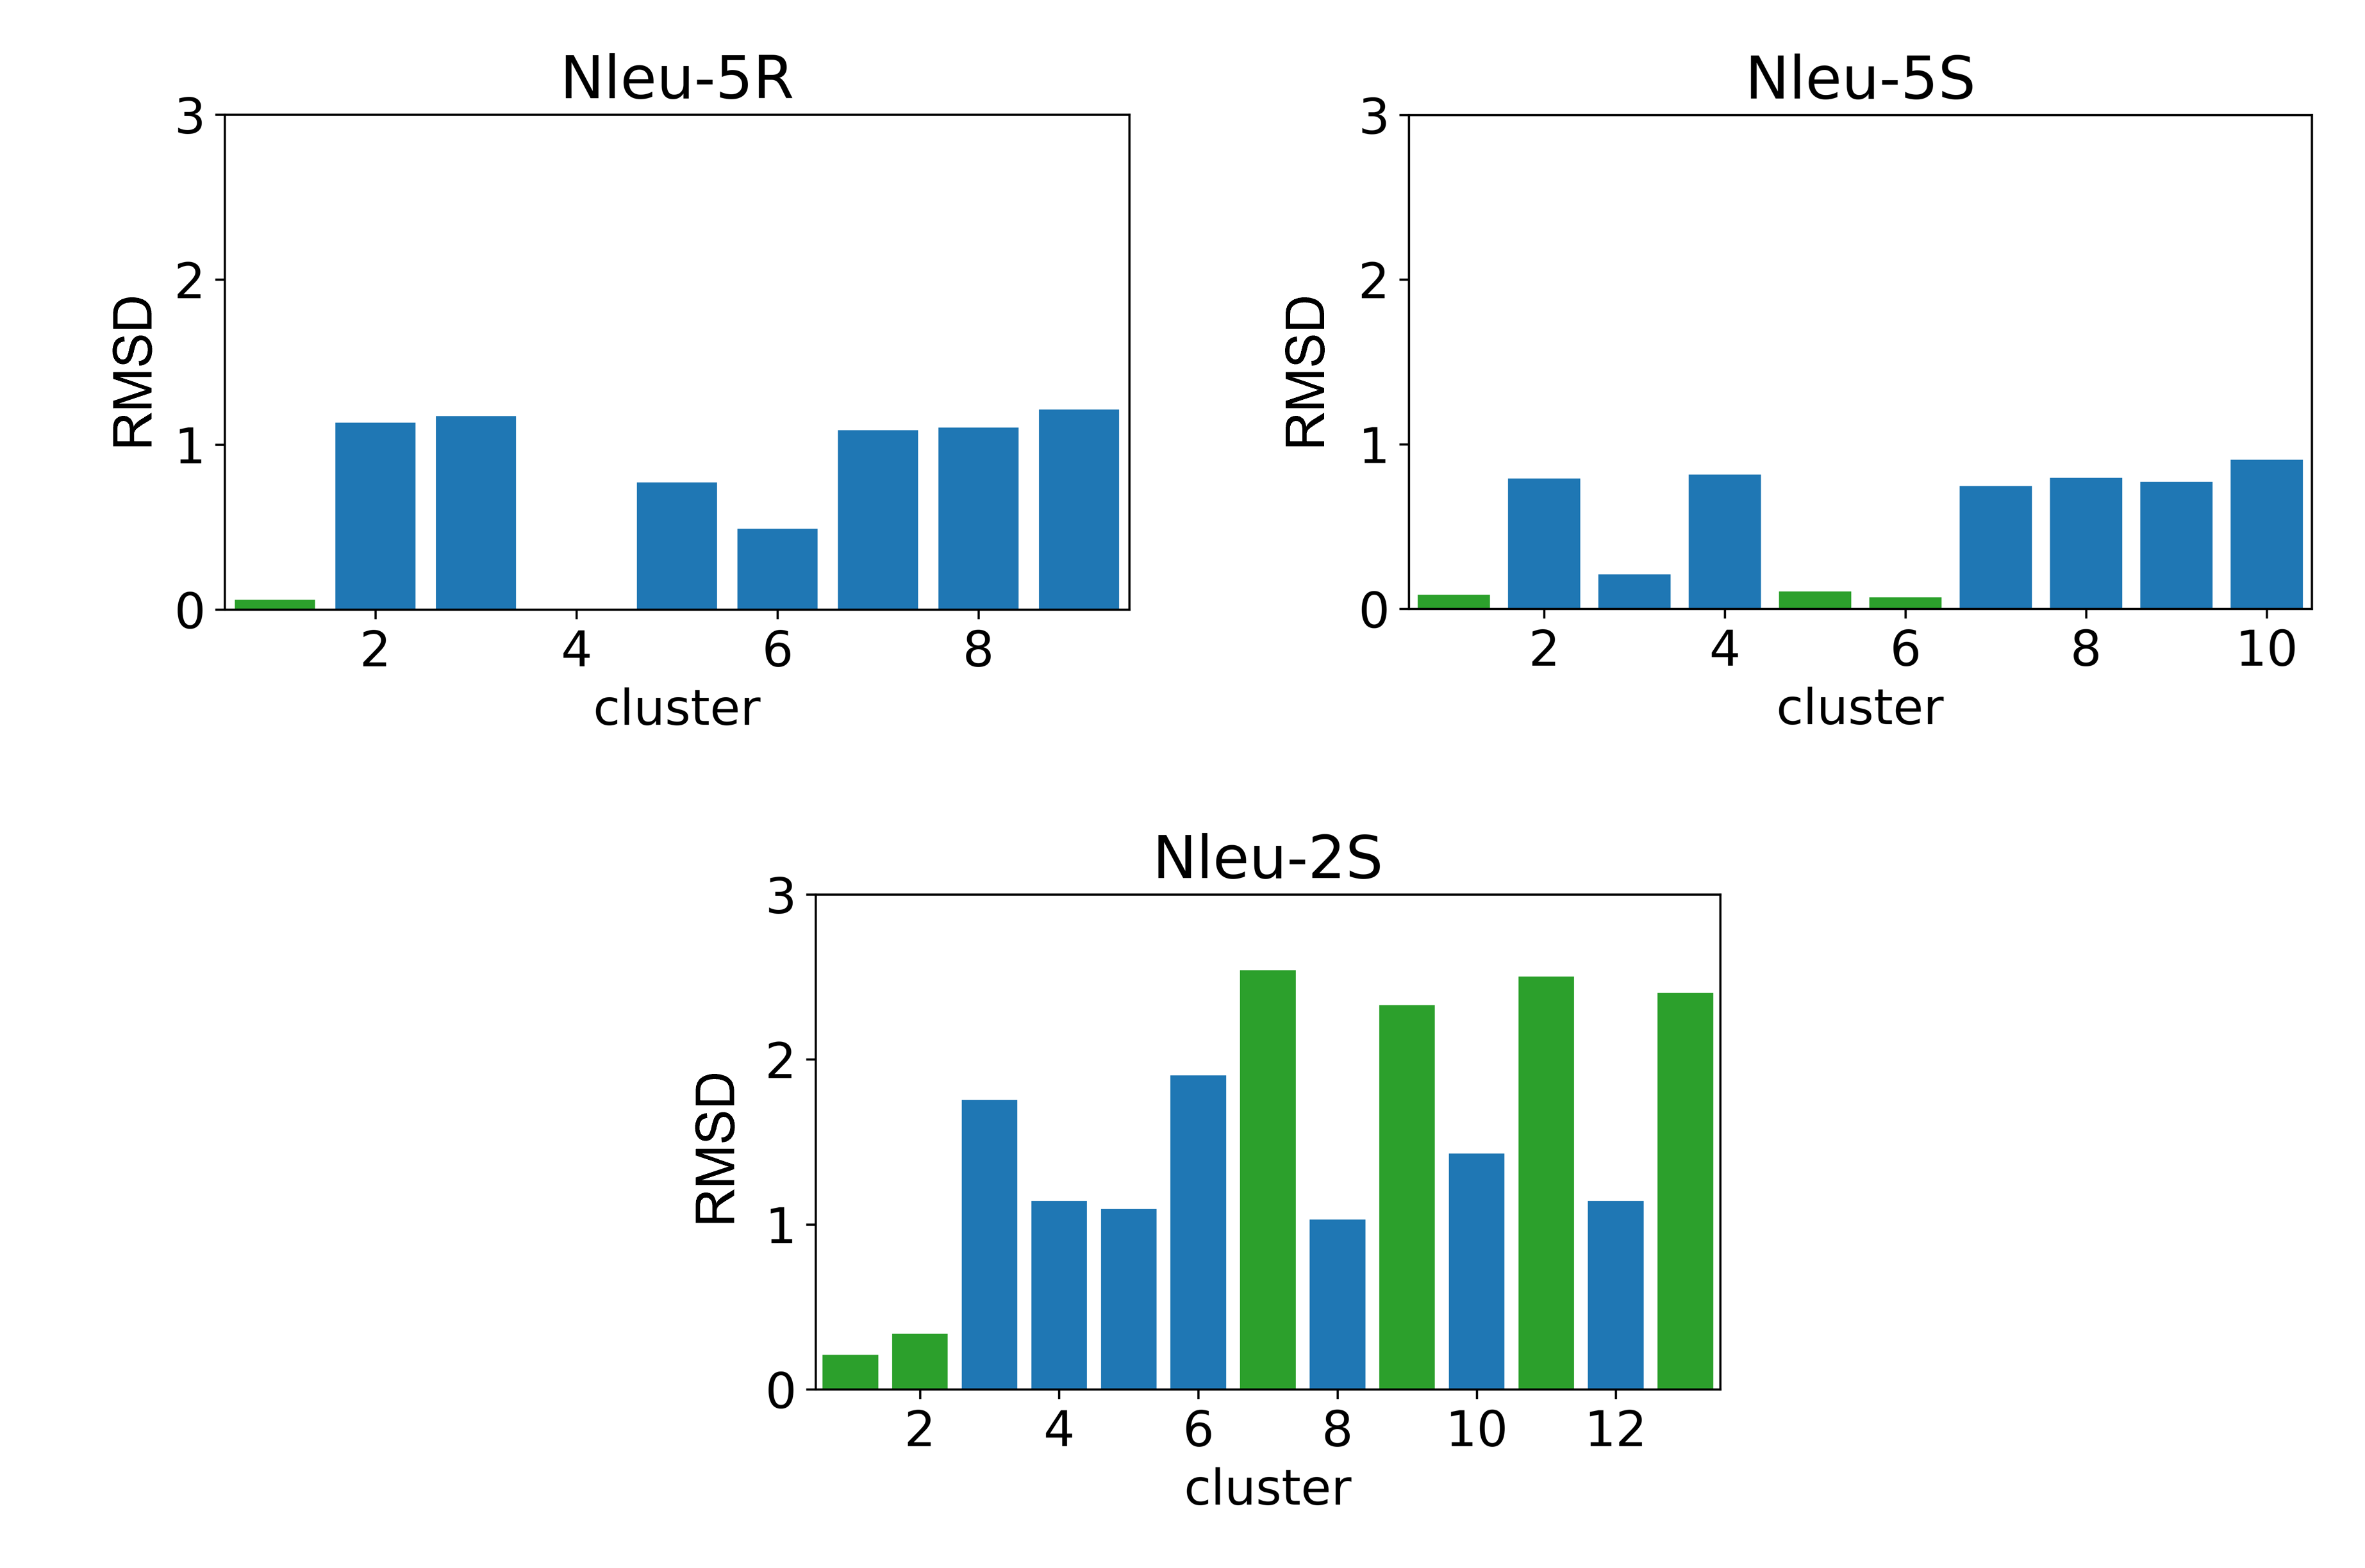
\includegraphics[width=\textwidth]{7_chapter_5/fig/results/j3NMRConfClusterAna.png}
    \caption{Root-mean-square deviation (RMSD, in hertz) between $^3$J$_{\text{HN–H}\alpha}$ coupling constants in chloroform from NMR measurements and from MD simulations. Clusters with the peptoid bond in trans conformation are shown in green.}
    \label{fig: j3NMRConfClusterAna}
\end{figure}

The clusters with all amides in trans conformation are in good agreement with the  $^3J_{\text{HN–H}\alpha}$ coupling constants (Figure \ref{fig: j3NMRConfClusterAna}), whereas the clusters containing the cis-peptoid bond deviate significantly from the experimental values. For Nleu-2R, the $^3J_{\text{HN–H}\alpha}$ coupling analysis is missing as we could not determine the $^3J_{\text{HN–H}\alpha}$ couplings reliably due to line broadening in the spectrum. The NOE-derived upper distance bounds are also generally reproduced in these clusters (Figures \ref{fig: SINOE violations Nleu-5S} -\ref{fig: SINOE violations Nleu-2SII}). Based on these findings, we focused the analysis in the following on those clusters, which have a reasonable agreement with the NMR data (i.e., clusters 1 and 4 for Nleu-5R, clusters 1, 5, and 6 for Nleu-5S, cluster 1 for Nleu-2R, and clusters 1 and 2 for Nleu-2S).

\begin{figure}[h!]
    \centering
    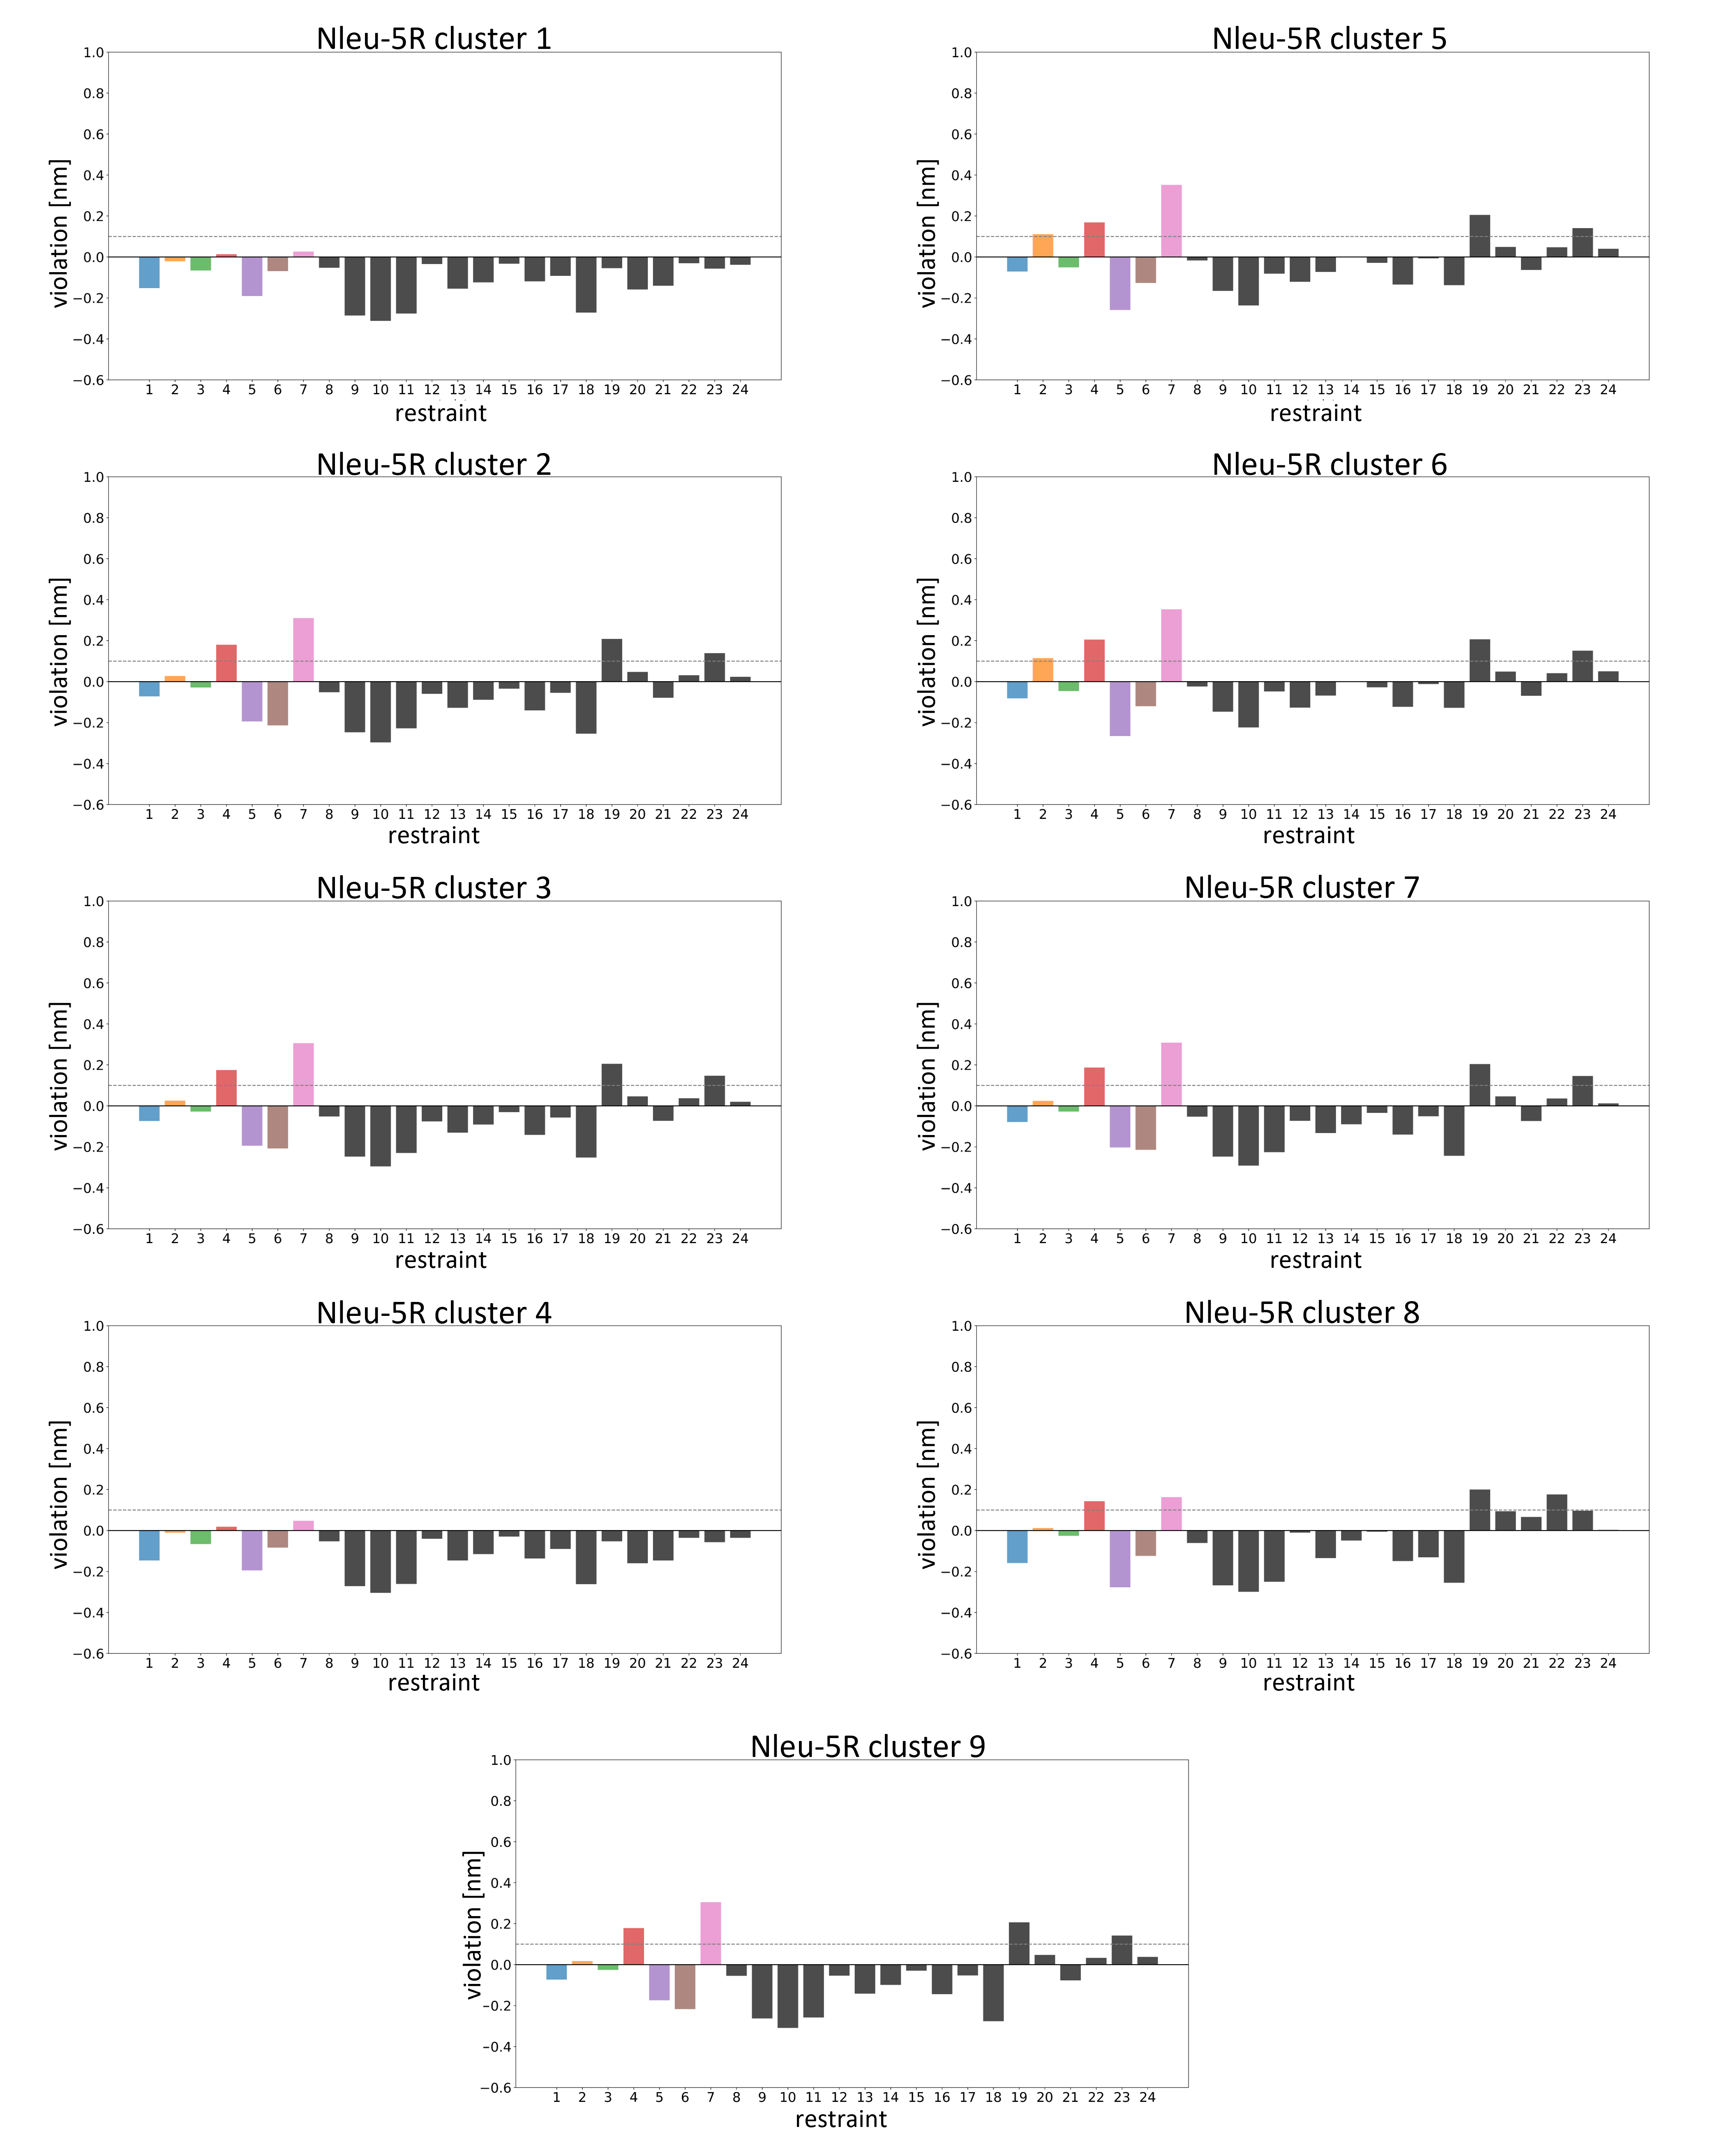
\includegraphics[width=\textwidth]{7_chapter_5/fig/results/NMR_5R.png}
    \caption{Violations of the NOE-derived upper distance bounds of Nleu-5R in chloroform by the clusters identified in the simulations in chloroform. Distances between residues across the backbone ring are colored. Distances between neighboring residues are shown in black. The dashed line indicates the expected uncertainty of the experimental upper bounds.}
    \label{fig: SINOE violations Nleu-5R}
\end{figure}

\begin{figure}[h!]
    \centering
    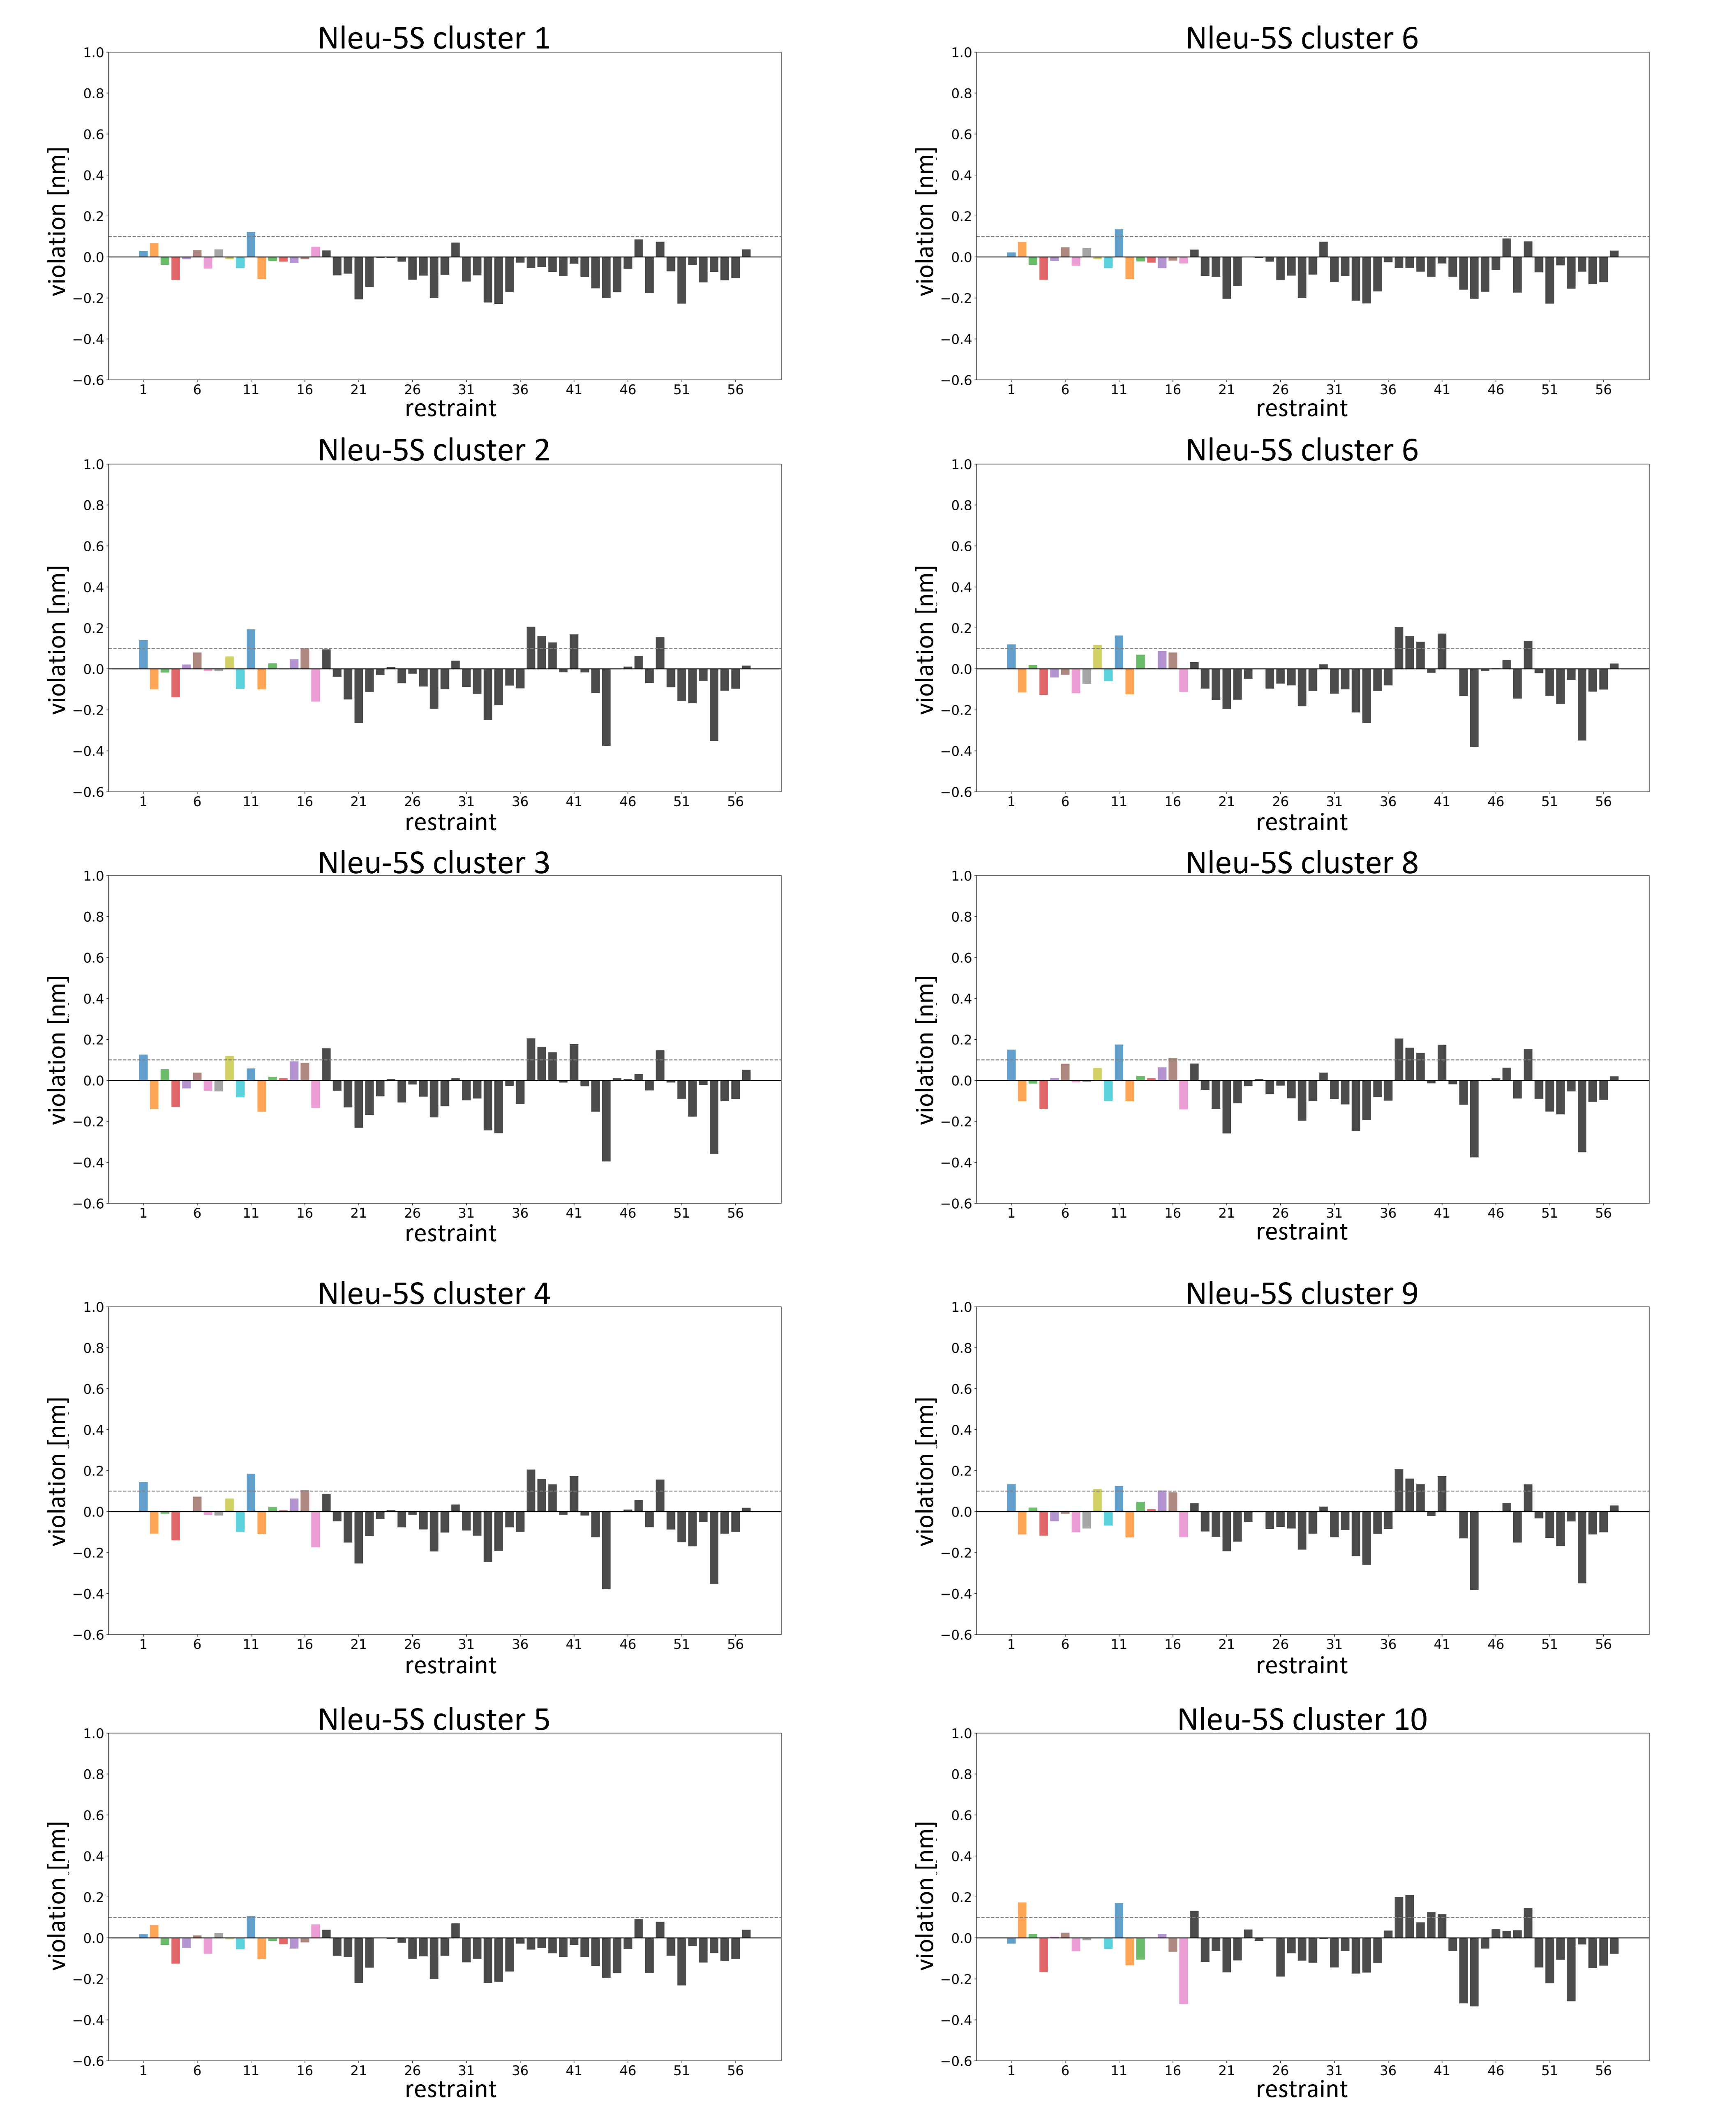
\includegraphics[width=\textwidth]{7_chapter_5/fig/results/NMR_5S.png}
    \caption{Violations of the NOE-derived upper distance bounds of Nleu-5S in chloroform by the clusters identified in the simulations in chloroform. Distances between residues across the backbone ring are colored. Distances between neighboring residues are shown in black. The dashed line indicates the expected uncertainty of the experimental upper bounds.}
    \label{fig: SINOE violations Nleu-5S}
\end{figure}

\begin{figure}[h!]
    \centering
    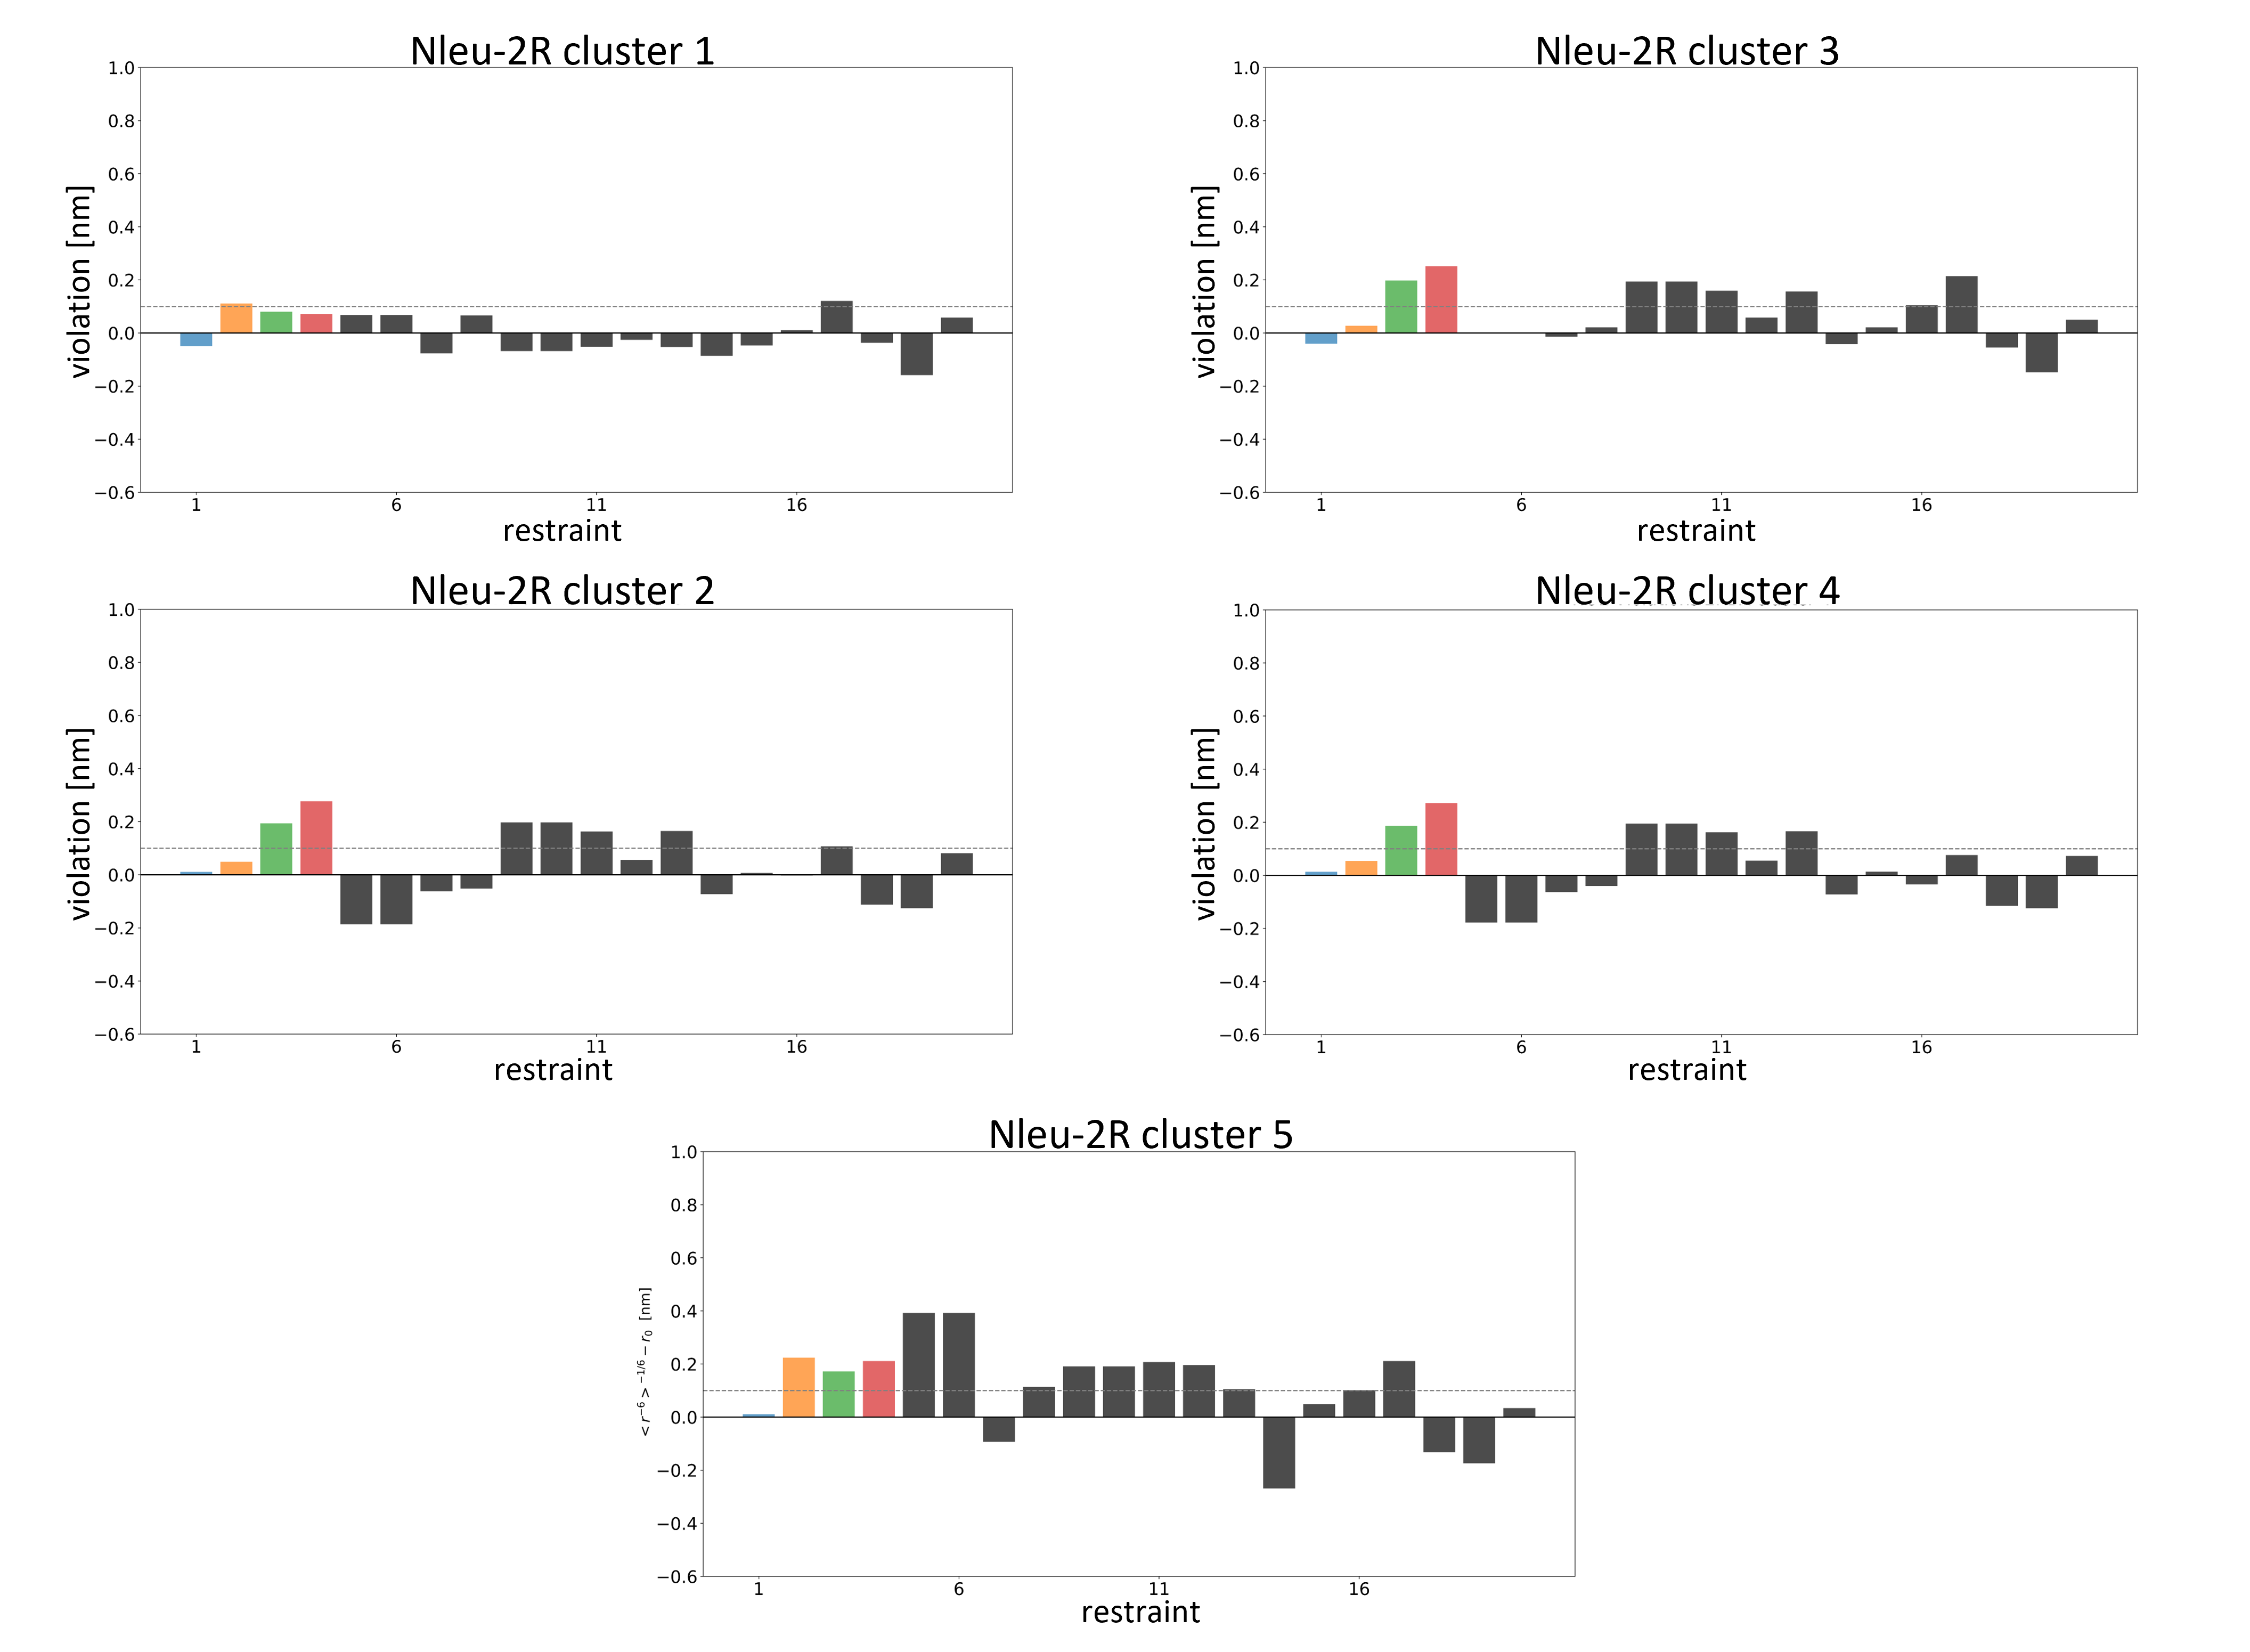
\includegraphics[width=\textwidth]{7_chapter_5/fig/results/NMR_2R.png}
    \caption{Violations of the NOE-derived upper distance bounds of Nleu-2R in chloroform by the clusters identified in the simulations in chloroform. Distances between residues across the backbone ring are colored. Distances between neighboring residues are shown in black. The dashed line indicates the expected uncertainty of the experimental upper bounds.}
    \label{fig: SINOE violations Nleu-2R}
\end{figure}

\begin{figure}[h!]
    \centering
    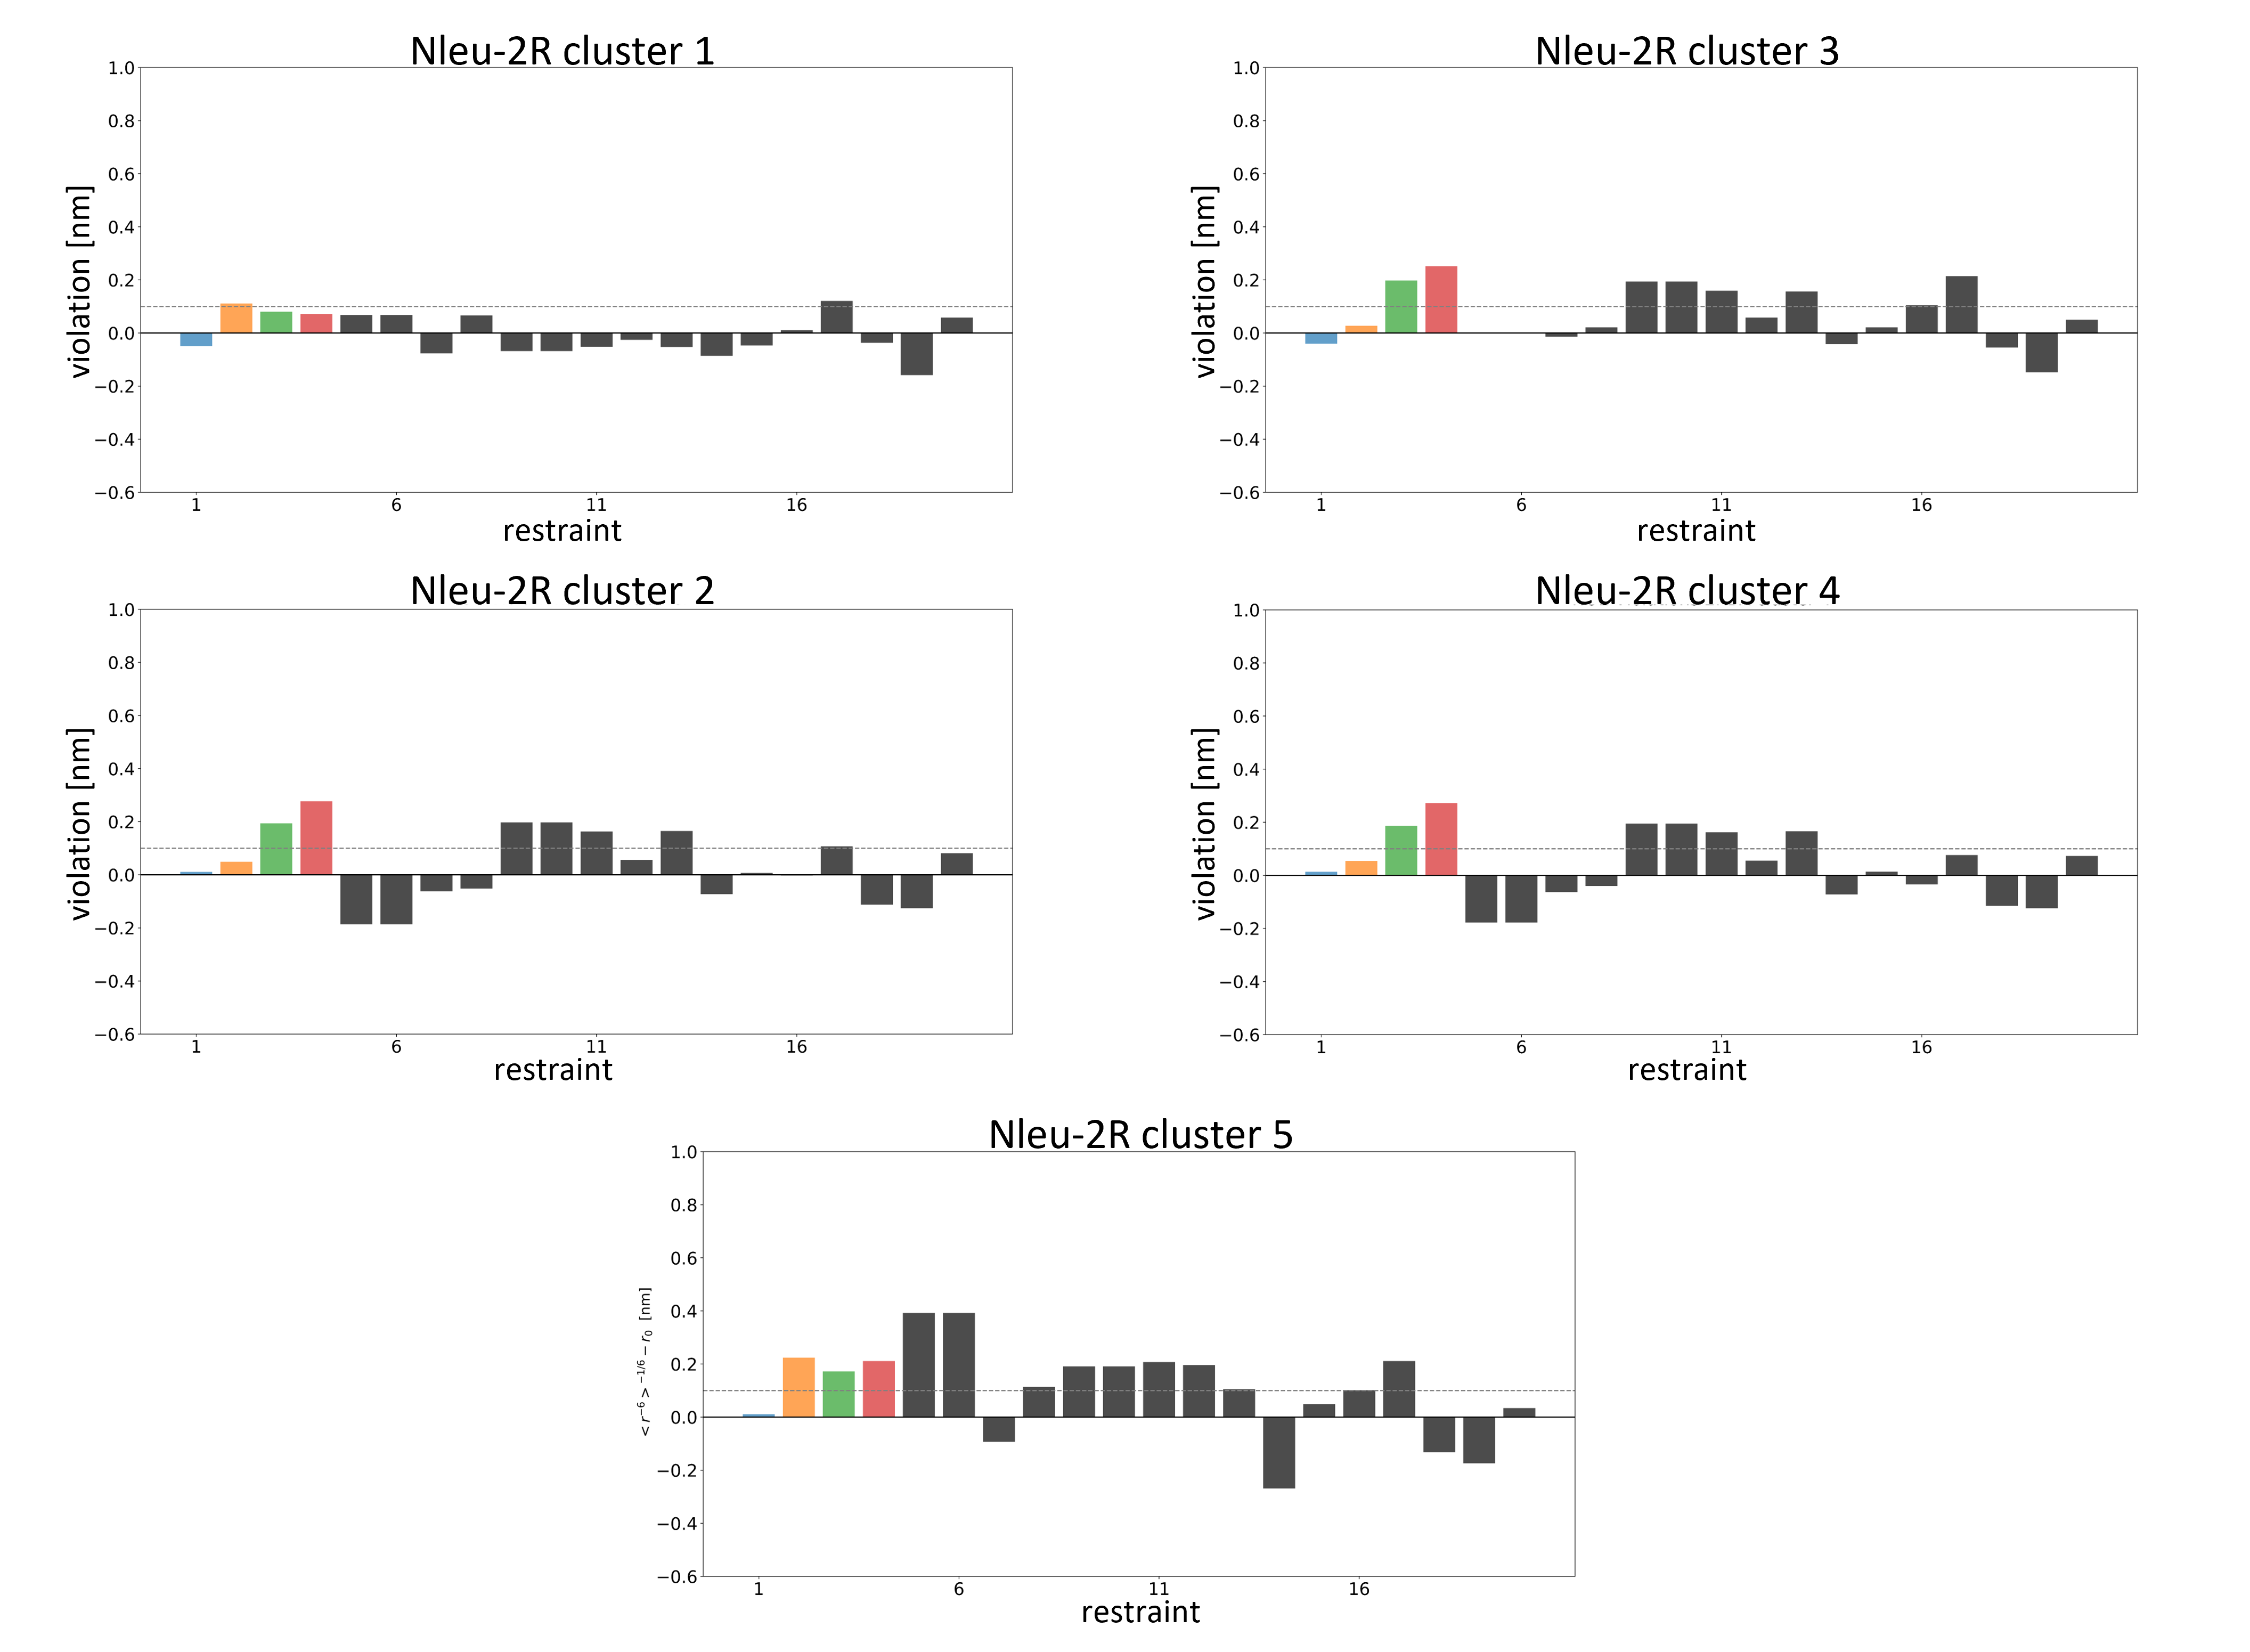
\includegraphics[width=\textwidth]{7_chapter_5/fig/results/NMR_2R.png}
    \caption{Violations of the NOE-derived upper distance bounds of Nleu-2S in chloroform by clusters 1–6 identified in the simulations in chloroform. Distances between residues across the backbone ring are colored. Distances between neighboring residues are shown in black. The dashed line indicates the expected uncertainty of the experimental upper bounds.}
    \label{fig: SINOE violations Nleu-2S}
\end{figure}

\begin{figure}[h!]
    \centering
    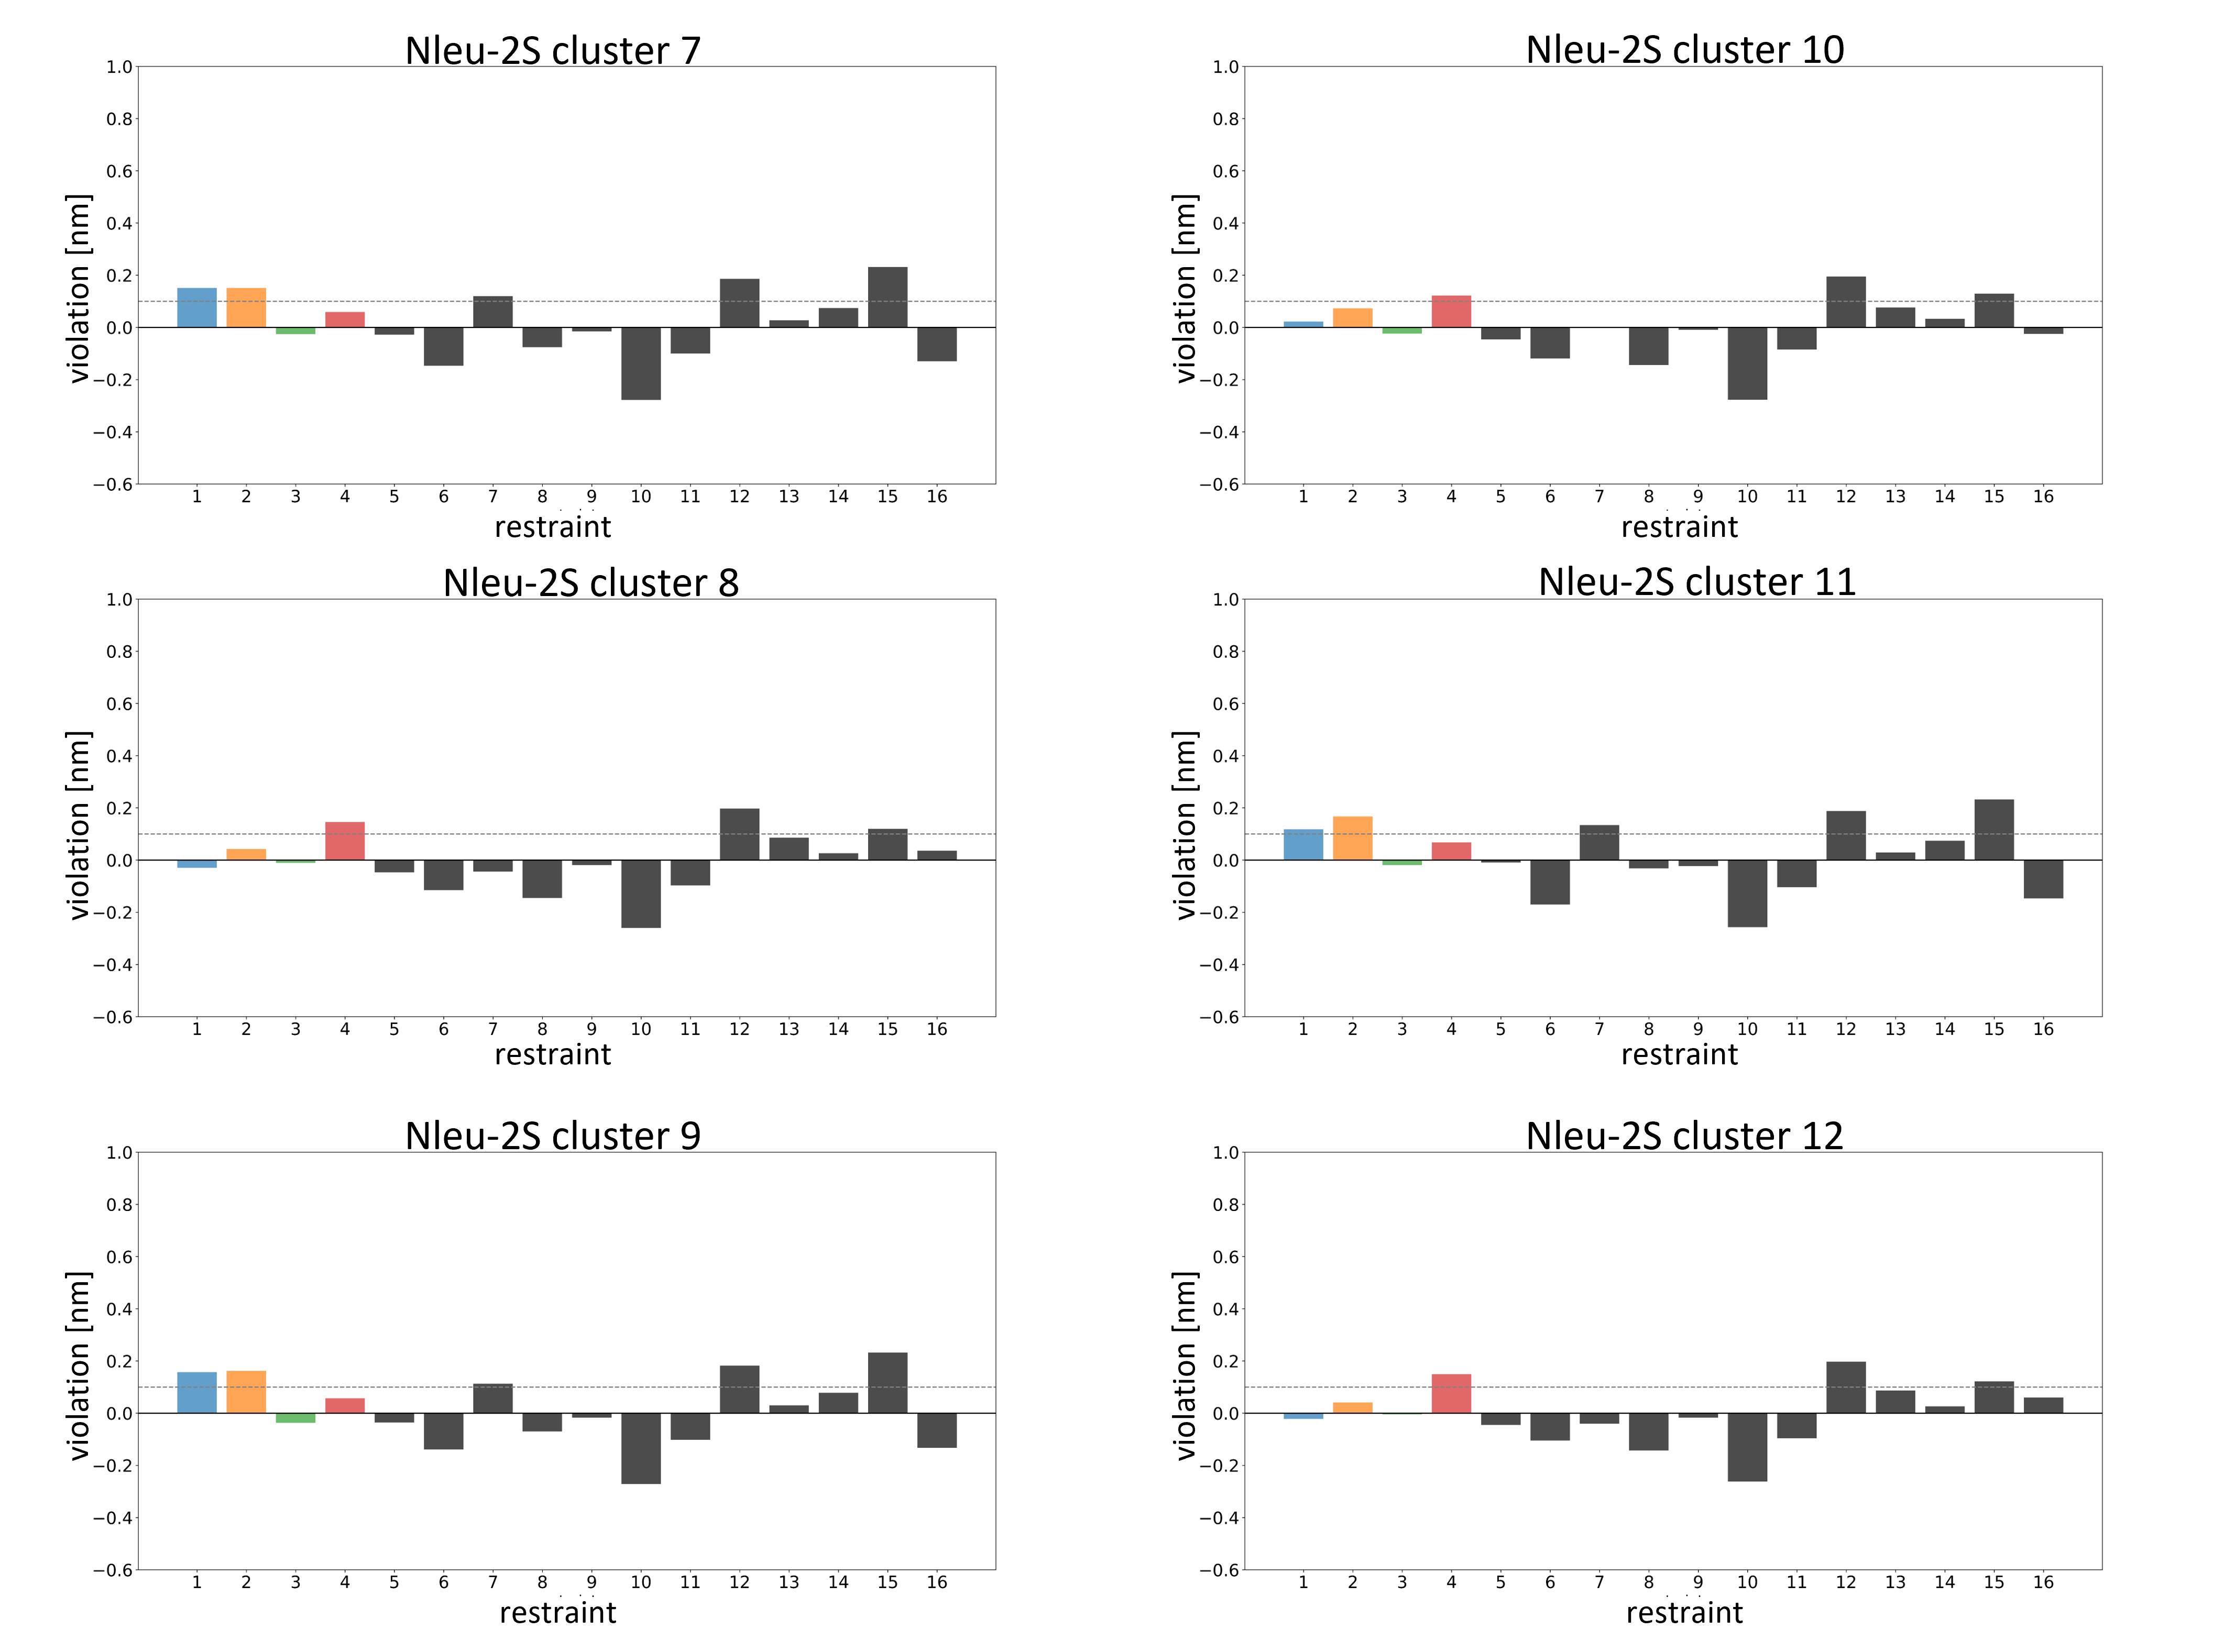
\includegraphics[width=\textwidth]{7_chapter_5/fig/results/NMR_2Sb.png}
    \caption{Violations of the NOE-derived upper distance bounds of Nleu-2S in chloroform by clusters 7–12 identified in the simulations in chloroform. Distances between residues across the backbone ring are colored. Distances between neighboring residues are shown in black. The dashed line indicates the expected uncertainty of the experimental upper bounds.}
    \label{fig: SINOE violations Nleu-2SII}
\end{figure}

\FloatBarrier
%-------------------------------------------

\subsection{Conformation Analysis}
A necessary condition for good membrane permeability is the adoption of conformations that shield polar groups optimally from the apolar environment. \cite{Sebastiano2018, Alex2011, Tyagi2018}
Therefore, we first analyzed the hydrogen-bonding patterns in the clusters in chloroform. For the peptides in this study, a maximum number of two H-bonds can be formed in a conformation due to ring strain. As can be seen in Table \ref{tab: hbondsratio}, the percentage of sampled conformations with two H-bonds differs significantly between Nleu-5R ($30\%$) and Nleu-5S ($7\%$). At the same time, the percentage of conformations without a H-bond is increased for Nleu-5S ($25\%$) compared to Nleu-5R ($8\%$). For the other pair, Nleu-2R and Nleu-2S, the percentages are more similar and in between those of Nleu-5R and Nleu-5S.


\begin{table}[h!]
    \centering
    \caption{Percentage of sampled conformations with zero, one, or two hydrogen bonds in chloroform. Analysis was restricted to the clusters with the trans-peptoid bond.}
    \label{tab: hbondsratio}
    \begin{adjustbox}{max width=\textwidth}
    \begin{tabular}{lccc}
    Number of hydrogen bonds [\%] &	0 &	1 &	2 \\
    \hline
    Nleu-5R  &	8	& 63	& 30 \\
    Nleu-5S  &	25	& 68	& 7  \\
    Nleu-2R  &	15	& 64	& 21 \\
    Nleu-2S  &	13	& 74	& 13 \\
    \hline
    \end{tabular}
    \end{adjustbox}
\end{table}

For a given molecule in an apolar environment, having access to conformations in which polar groups are shielded -- such as by H-bonding -- should be energetically favorable. 
To assess this effect, we extracted the potential energy of the peptides (i.e., intramolecular and peptide-solvent contributions) from the trajectories. 
The normality of each potential-energy distribution was confirmed by the Shapiro–Wilk test \cite{Shapiro1965} (Table \ref{tab: SIstatTestingNorm}). 

\begin{table}[h!]
\centering
\caption{Average potential energy of the peptides (i.e., sum of the intramolecular $\langle \text{V} \rangle$ contributions and the peptide–solvent contributions)  together with the $p$-value of the Shapiro-Wilk test for the simulations in chloroform and water, respectively. The significance limit for the $p$-value was 0.05.}
\label{tab: SIstatTestingNorm}
\begin{adjustbox}{max width=\textwidth}
\begin{tabular}{r|cc|cc}
\multirow{2}{*}{Molecule} & \multicolumn{2}{l}{Chloroform} & \multicolumn{2}{l}{Water}        \\
    & $\langle \text{V} \rangle [\text{kJ}/\text{mol}]$ & $\text{p}_{\text{Shapiro-Wilk}}$ & $\langle \text{V} \rangle [\text{kJ}/\text{mol}]$ & $\text{p}_{\text{Shapiro-Wilk}}$  \\
    \hline
    Nleu-5R    & -217.08    & \~0.0          & -117.77  & \~0.0         \\
    Nleu-5S    & -208.39    &   $5.9*10^{-8}$  & -115.64  & $5.24*10^{-10}$ \\
    Nleu-2R    & -211.17    & \~0.0          & -117.84  & \~0.0         \\
    Nleu-2S    & -216.63    &   $7.6*10^{-39}$ & -116.91  & \~0.0   \\
    \hline
\end{tabular}%
\end{adjustbox}
\end{table}

\begin{table}[h!]
\centering
\caption{Results of the Fisher t-test to validate the significance of the deviations in the average potential energy of the peptides. The significance limit for the $p$-value was 0.05.}
\label{tab: SIstatTestingDiff}
\begin{adjustbox}{max width=\textwidth}
\begin{tabular}{lcc}
Molecule          & Chloroform & Water     \\
\hline
Nleu-5R - Nleu-5S & $\sim$0.0  & $\sim$0.0 \\
Nleu-2R - Nleu-2S & $\sim$0.0  & $2.7*10^{-77}$\\
\hline
\end{tabular}%
\end{adjustbox}
\end{table}

The Fisher t-test \cite{Kotz1998} was employed to determine if the means of the distributions differ statistically significantly ($p < 0.05$). 
This was found to be the case for each pair of distributions (Table \ref{tab: SIstatTestingDiff}). 
On average, the potential energy of Nleu-5R is $9$~kJ/mol lower (i.e., more favorable) in chloroform compared to Nleu-5S, whereas the difference in the average potential energy between Nleu-2R and Nleu-2S is $6$~kJ/mol. In many studies in the literature, it was found that the 3D-PSA is a good measure for the degree of polar shielding in conformations. \cite{Roux2020, Sebastiano2018, Vorherr2018, Peraro2018} 
However, for the present set of four peptides, no correlation was observed between the 3D-PSA and the potential energy (Figure \ref{fig: SI3DPSAANA}). 
The ring strain in the relatively small backbone cycle of the peptides affects the geometry of the intramolecular H-bonds, which is likely not reflected appropriately in the 3D-PSA calculation. 
\begin{figure}[h!]
    \centering
    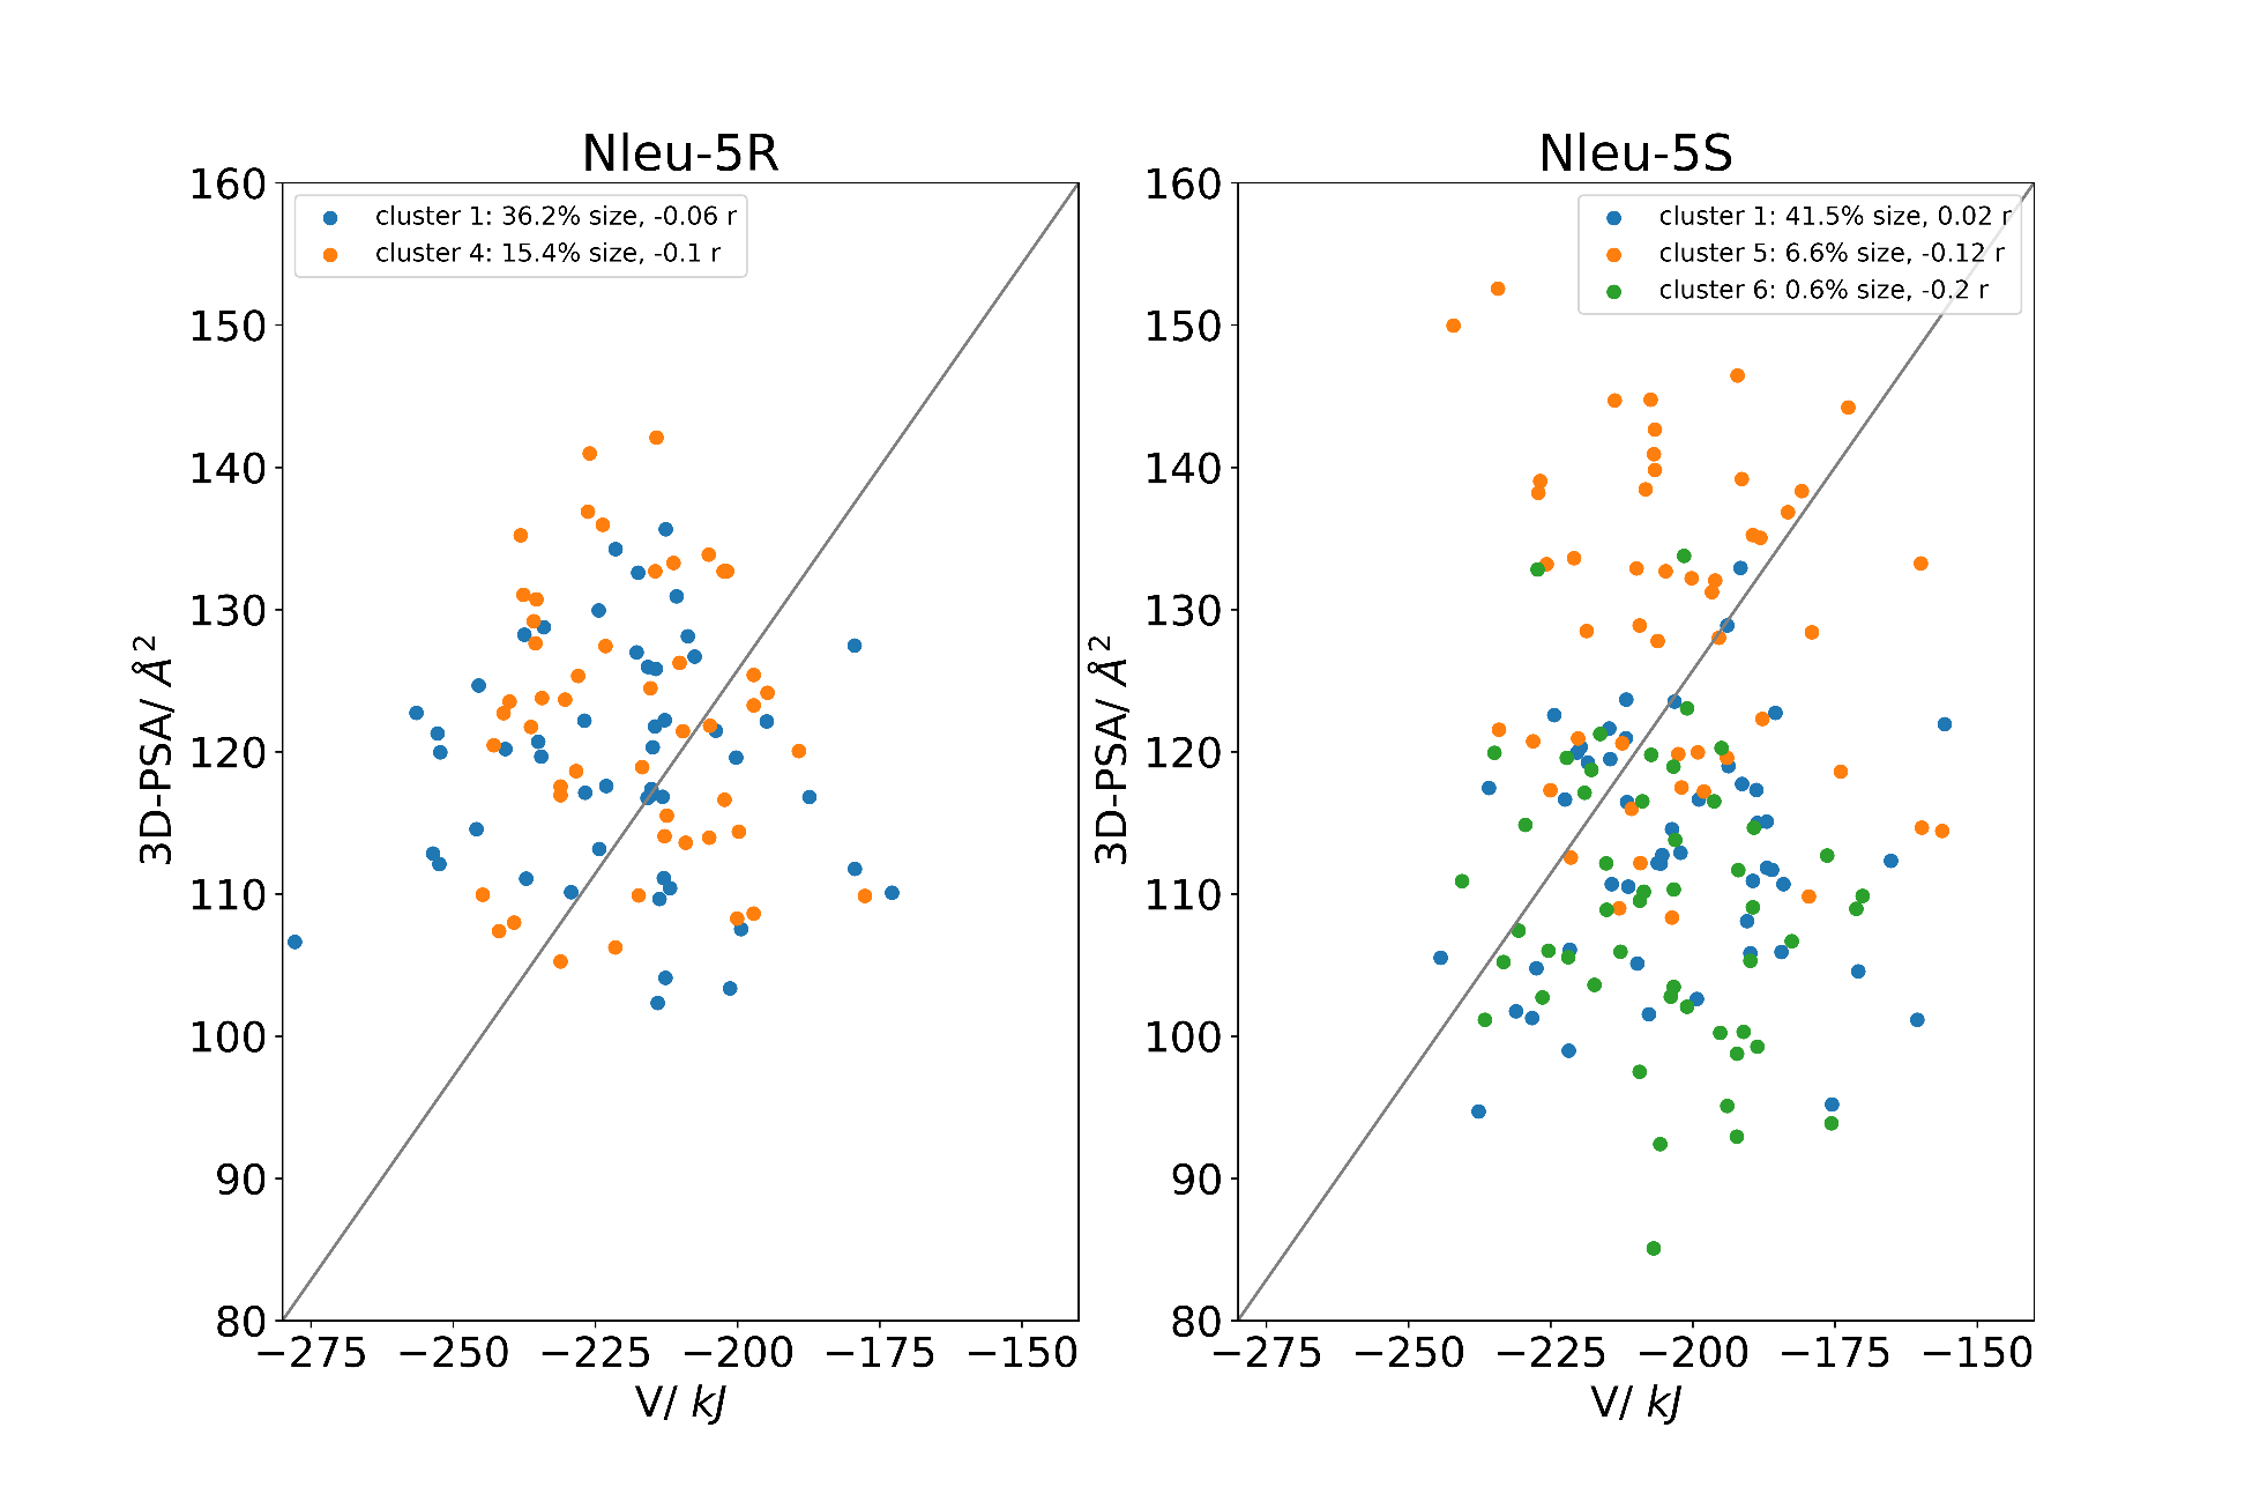
\includegraphics[width=\textwidth]{7_chapter_5/fig/results/3dPSA.png}
    \caption{Correlation between the 3D-PSA and the potential energy of the corresponding conformation (i.e., sum of intramolecular contributions and peptide–solvent contributions) for Nleu-5R and Nleu-5S in chloroform. The 100 structures closest to the cluster center were taken for the clusters with the trans-peptoid bond. The trend for an expected linear correlation is shown as gray line. The legend contains the cluster population in percentage and the Spearman correlation coefficient $r$.}
    \label{fig: SI3DPSAANA}
\end{figure}

In summary, the ranking Nleu-5R $<$ Nleu-2S $<$ Nleu-2R $<$ Nleu-5S, which was found in terms of both hydrogen-bonding patterns and potential energies, matches well with the experimental permeability data.
The findings described above indicate that the change in stereochemistry of the methyl group in position $5$ between Nleu-5R and Nleu-5S leads to different conformational behavior. 
A detailed analysis of the H-bonds showed that only Nleu-5S forms a H-bond between Ala-O and the tether-NH with an occurrence of $24\%$ in chloroform (Table \ref{tab: hbondsrationCLCH3}). 
This H-bond across the ring of Nleu-5S prevents the formation of other H-bonds (Figure \ref{fig: HbondExamples}B).
Such a conformation with a single H-bond is likely less favorable (compared to one with more H-bonds) in chloroform because less polar groups are shielded. In the dominant conformation of Nleu-5R, on the other hand, two H-bonds can be formed across the ring (Figure \ref{fig: HbondExamples}A).

\begin{figure}[h!]
    \centering
    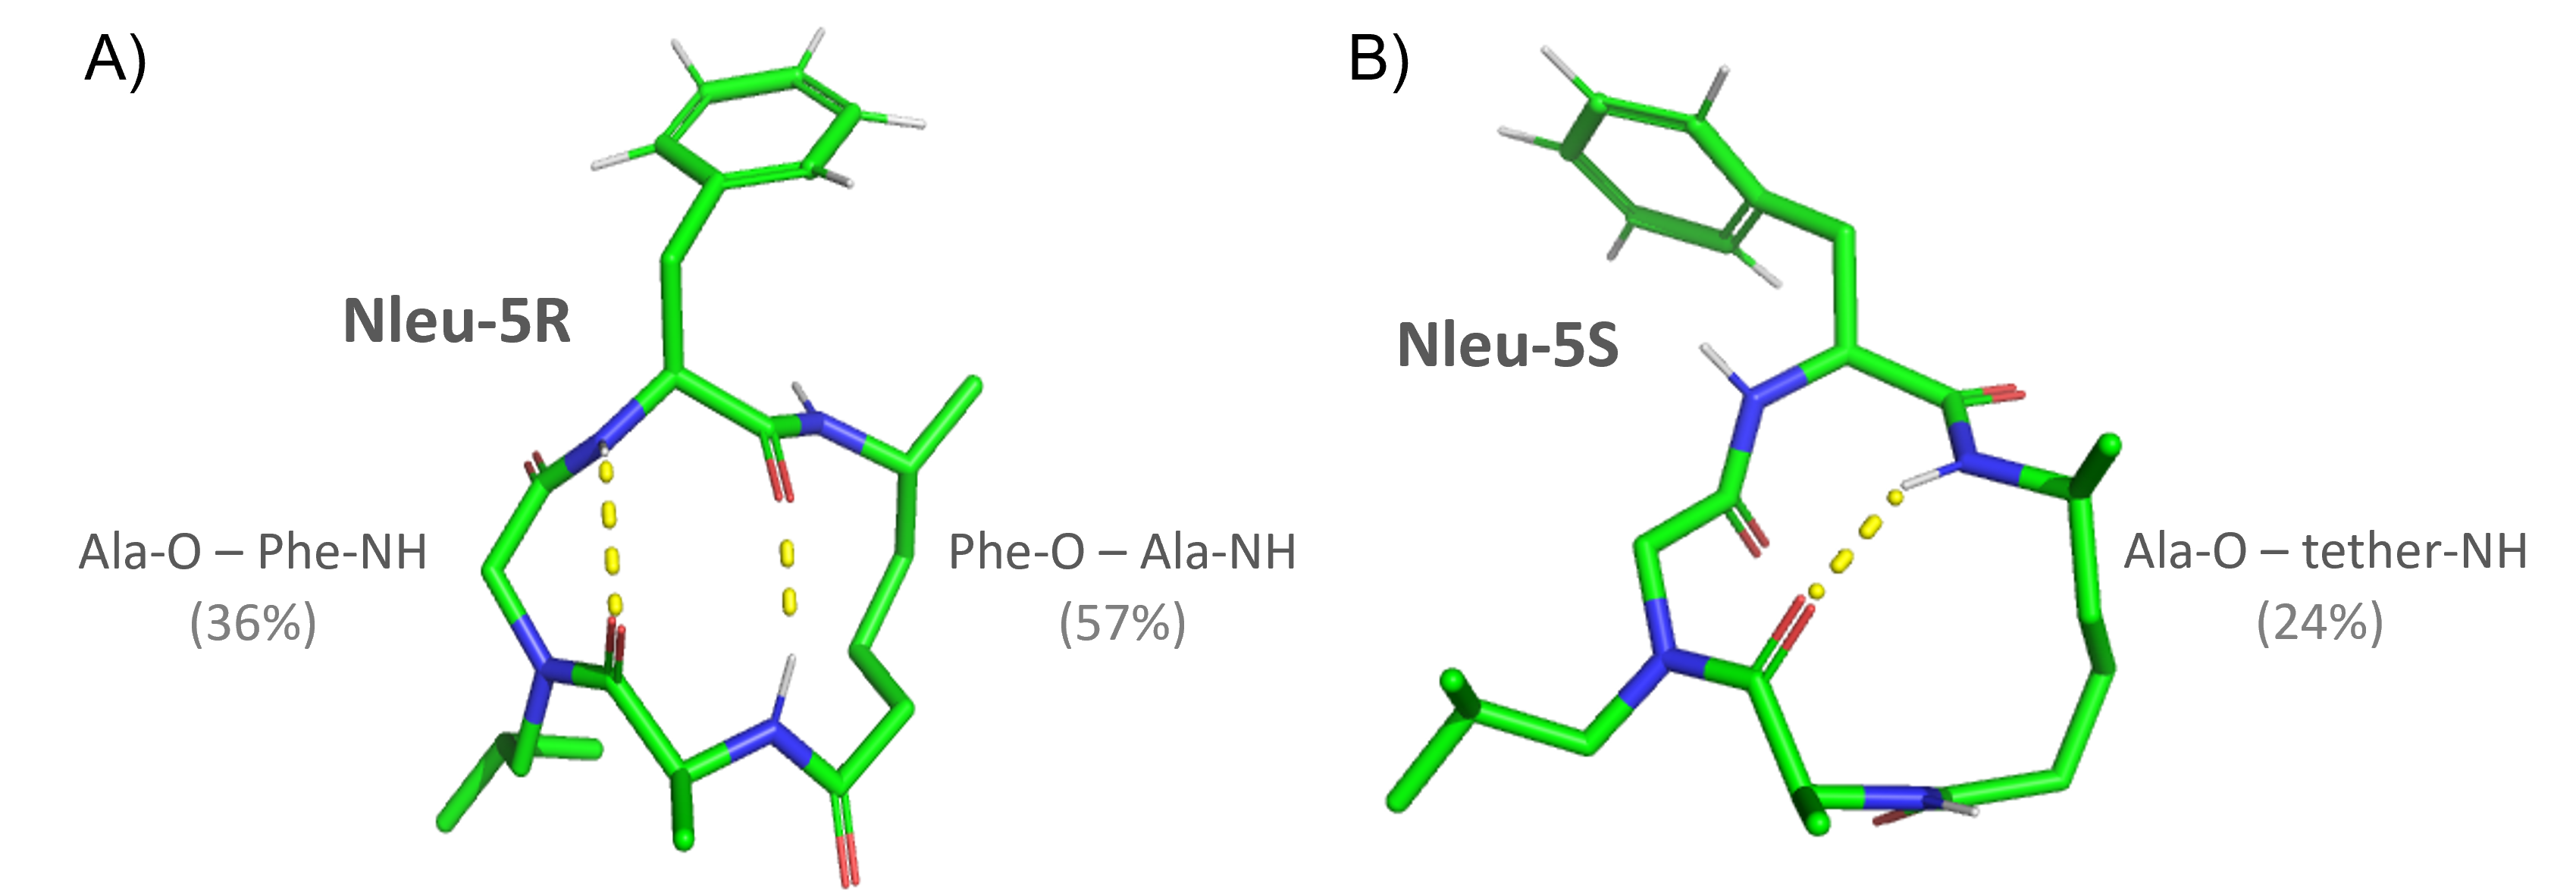
\includegraphics[width=\textwidth]{fig/results/ExampleHbonds.png}
    \caption{Snapshots of Nleu-5R (\textbf{A}) and Nleu-5S (\textbf{B}) from MD simulations in chloroform. Hydrogen bonds are shown with their percentage of the absolute occurrence in chloroform in the trans-peptoid clusters. Pictures were generated with PyMol. \cite{Delano2020}}
    \label{fig: HbondExamples}
\end{figure}

\begin{table}[h!]
    \centering
    \caption{Hydrogen bond occurrence in percentage for the sampled conformations in chloroform. Analysis was restricted to the clusters with the trans-peptoid bond.}
    \label{tab: hbondsrationCLCH3}
    \begin{adjustbox}{max width=\textwidth}
    \begin{tabular}{lcccc}
    H-bond  [\%] &	Nleu-2R &	Nleu-2S &	Nleu-5R &	Nleu-5S  \\
    \hline
    Nleu-O tether-NH &	74 &	37 &	28 &	33 \\
    Ala-O tether-NH &	\textless{}1 & \textless{}1 &	\textless{}1 &	24 \\
    Phe-O Ala-NH    &	\textless{}1 &	35 &	57 &	\textless{}1 \\
    Ala-O Phe-NH    &	27 &	25 &	36 &	17 \\
    \hline\\
    \end{tabular}
    \end{adjustbox}
\end{table}

Next, we analyzed the torsional-angle distributions in the backbone ring of the peptides. The change in stereochemistry of the methyl group at position 5 leads to a shift in the torsional-angle distributions of the tether units for Nleu-5S compared to Nleu-5R (Figure \ref{fig: dihedralDist}A). This shift results in a bent conformation of the ring (Figure \ref{fig: dihedralDist}B), which allows only one H-bond to form between Ala-O and tether-NH (Figure \ref{fig: dihedralDist}B). There is also a shift in the backbone torsional-angle distributions between Nleu-2R and Nleu-2S, however, to a much smaller extent (Figure \ref{fig: SITorsion2RS}). Noteably a longrange effect in the dihedral distribution for the phenylalanine residue was detected. The missing hydrogen bond and the resulting rotation of the carbonyl group seem to hinder the free rotation of the phenylalanine rest (Figure \ref{fig: dihedralDistSubst}).

\begin{figure}[h!]
    \centering
    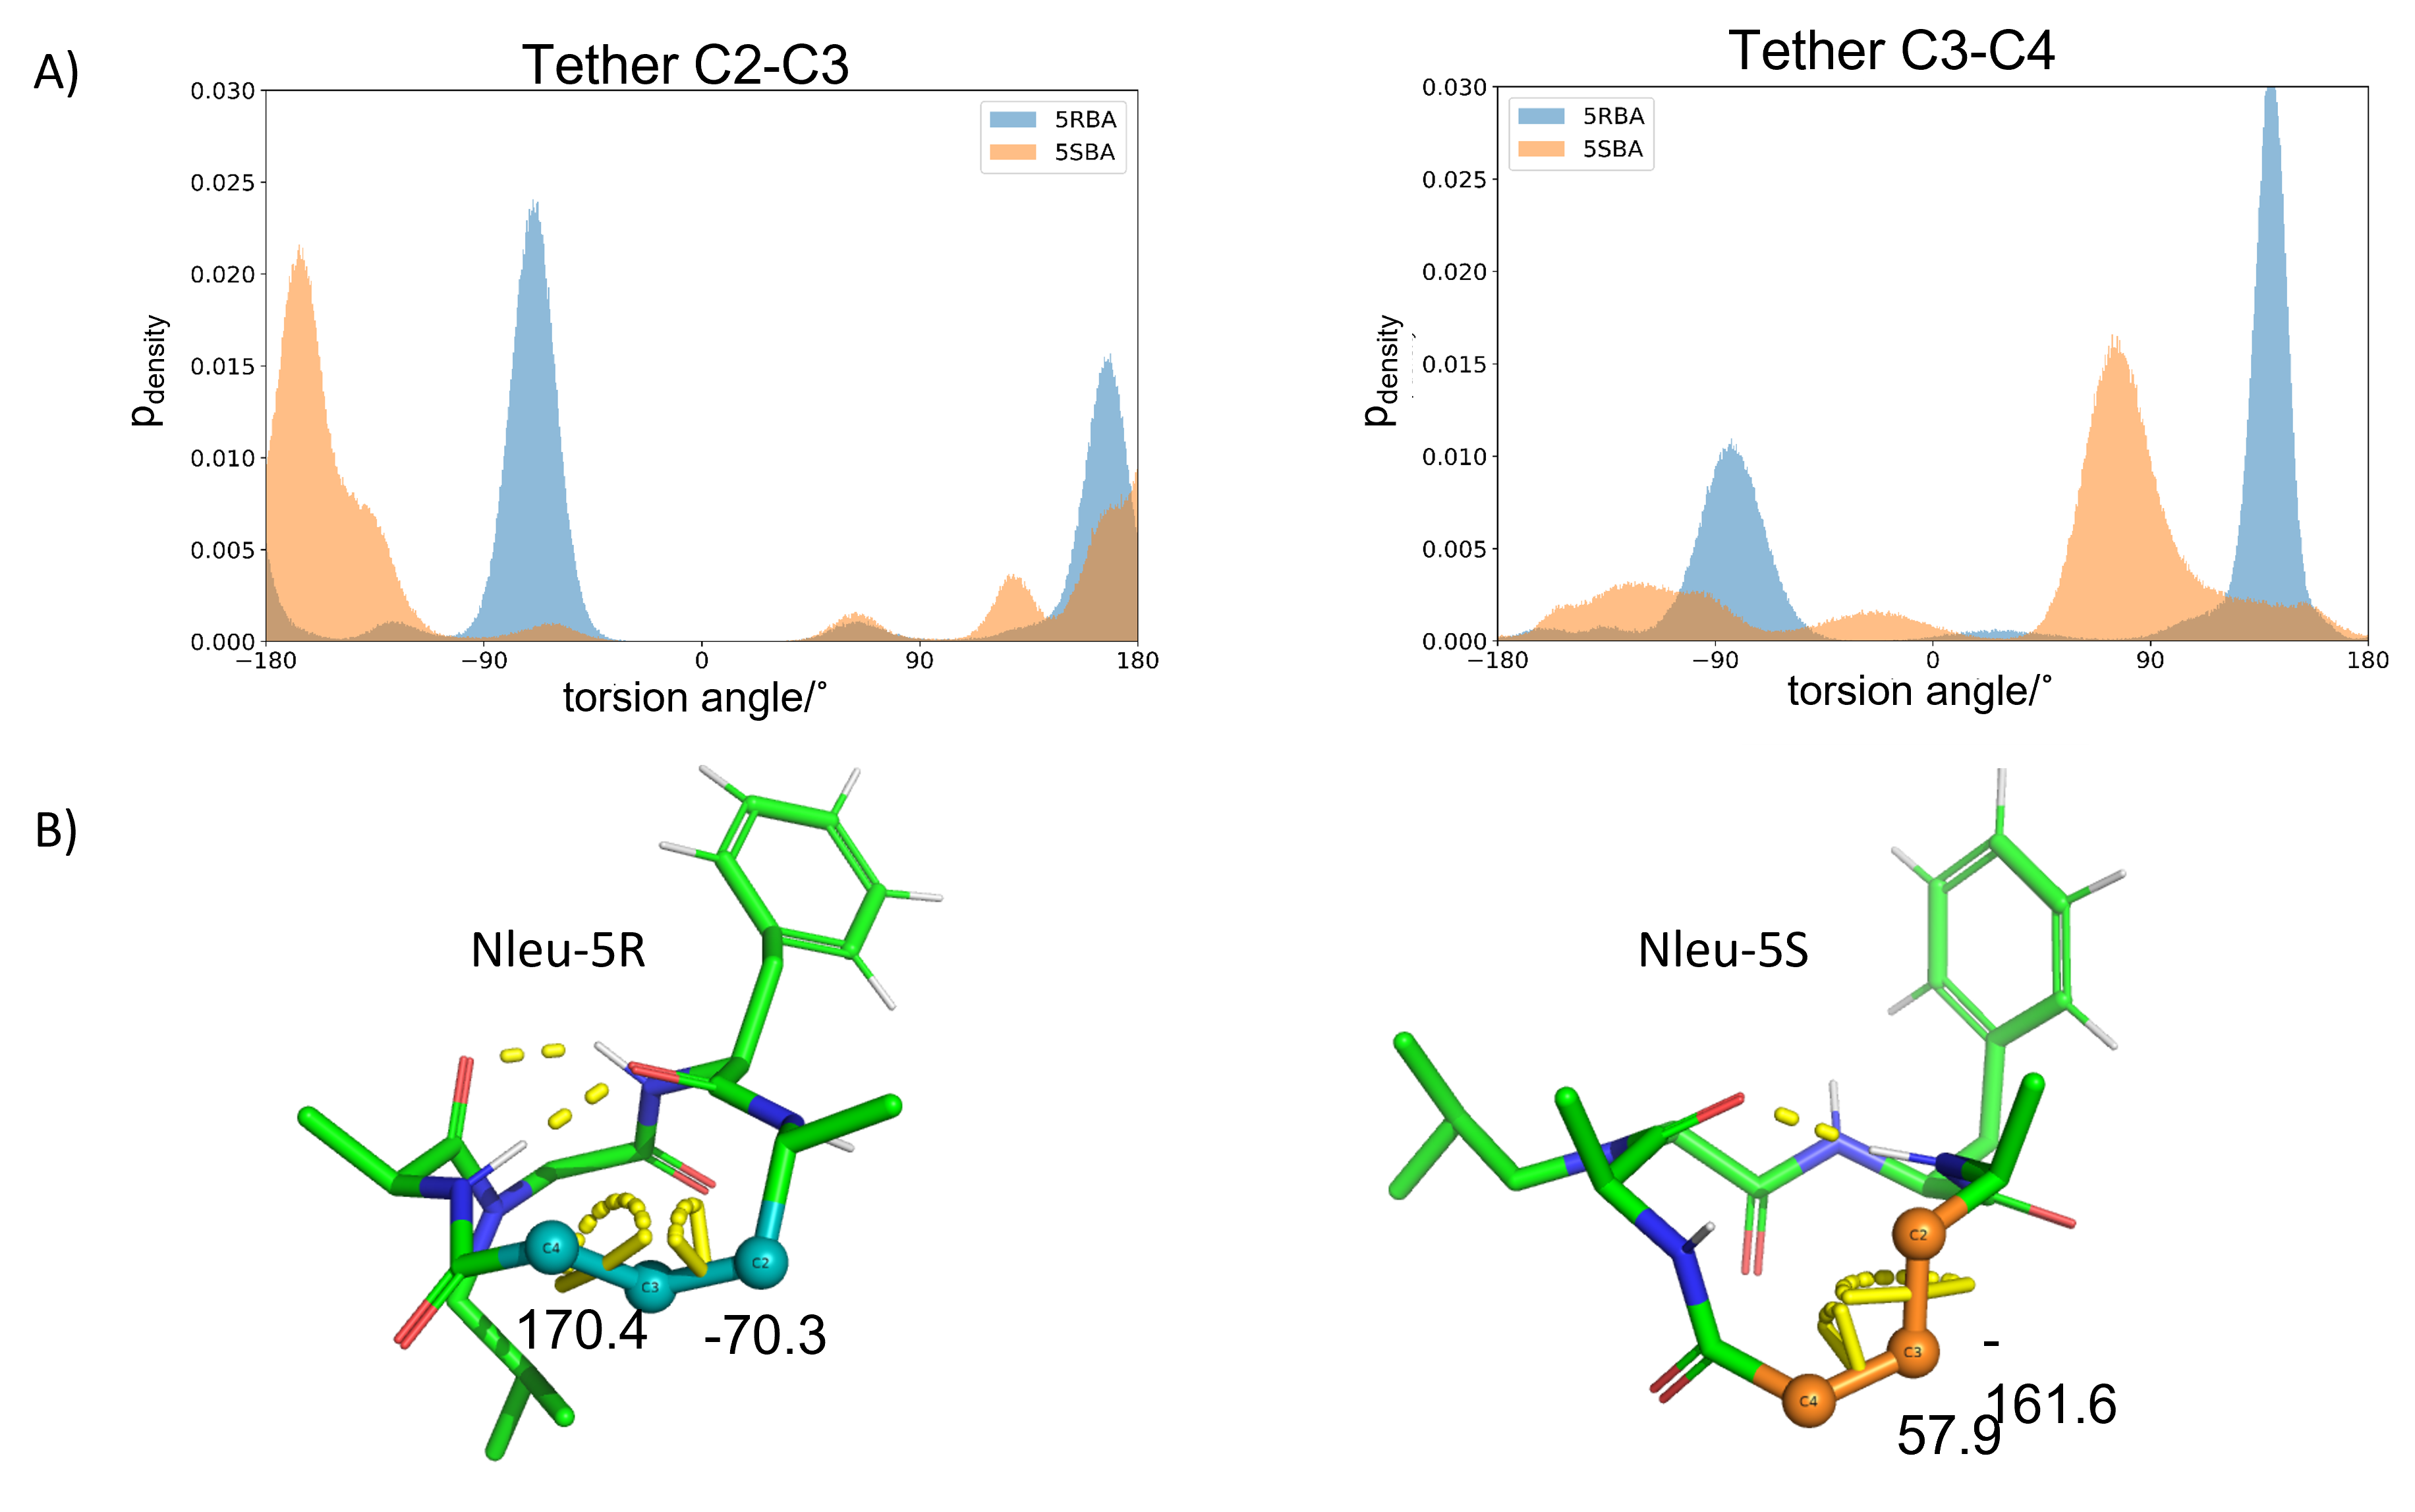
\includegraphics[width=\textwidth]{7_chapter_5/fig/results/dihedral_dist.png}
    \caption{(\textbf{A}) Torsional-angle distributions of the tether in Nleu-5R (blue) and Nleu-5S (orange) in chloroform. The analysis was restricted to the clusters with the trans-peptoid bond. (\textbf{B}) Torsional angles of the tether (shown in cyan and orange) corresponding to the peaks of the distributions. Pictures were generated with PyMol. \cite{Delano2020} The change in the stereocenter also affects the $\chi_1$-angle of the phenylalanine residue as the tether conformation hinders the rotation around this torsion due to a steric clash with the carbonyl group that is facing out of the backbone ring (Figure \ref{fig: dihedralDistSubst}).
    }
    \label{fig: dihedralDist}
\end{figure}

\begin{figure}[h!]
    \centering
    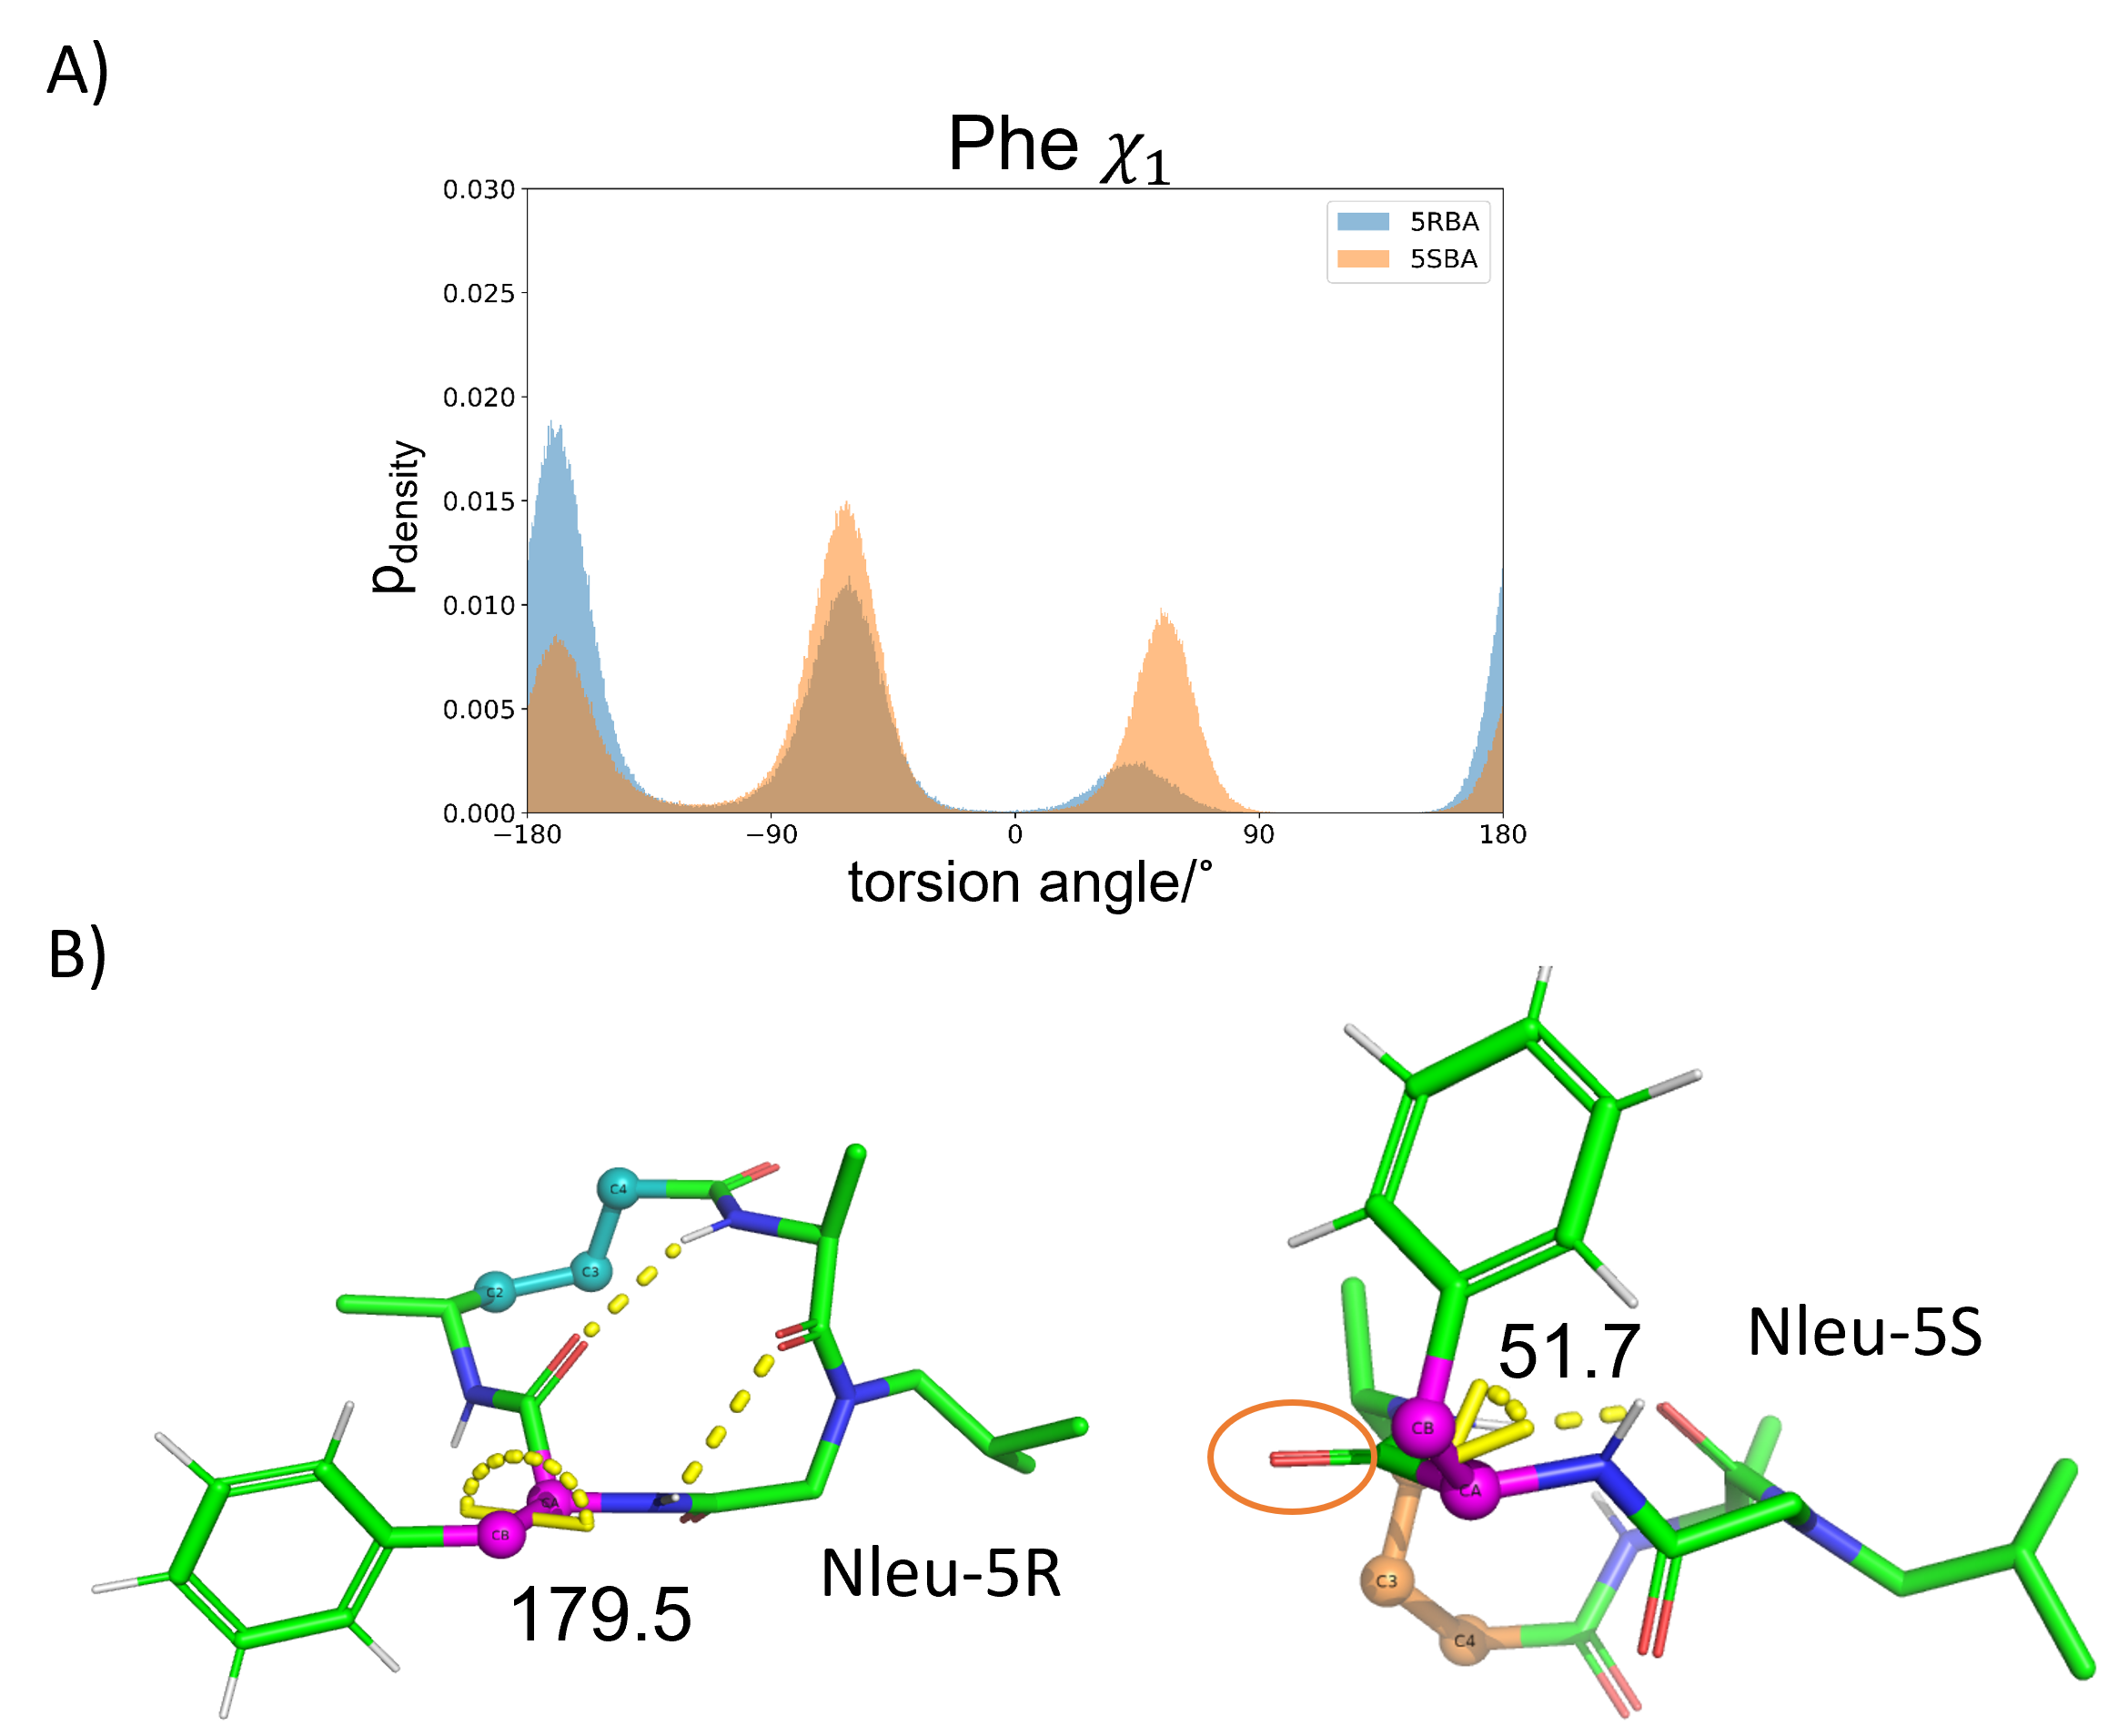
\includegraphics[width=\textwidth]{7_chapter_5/fig/results/dihedral_dist_subs.png}
    \caption{(\textbf{A}) Torsional-angle distributions of the $\chi_1$ torsional angle of the phenylalanine residue in Nleu-5R (blue) and Nleu-5S (orange) in chloroform. Analysis was restricted to the clusters with the trans-peptoid bond. (\textbf{B}) $\chi_1$ torsional angle of the phenylalanine residue (shown in purple) corresponding to the peaks of the distributions. The backbone carbonyl interferes with the rotation around this torsion is highlighted with a red circle. Pictures were generated with PyMol. \cite{Delano2020}}
    \label{fig: dihedralDistSubst}
\end{figure}

\begin{figure}[h!]
    \centering
    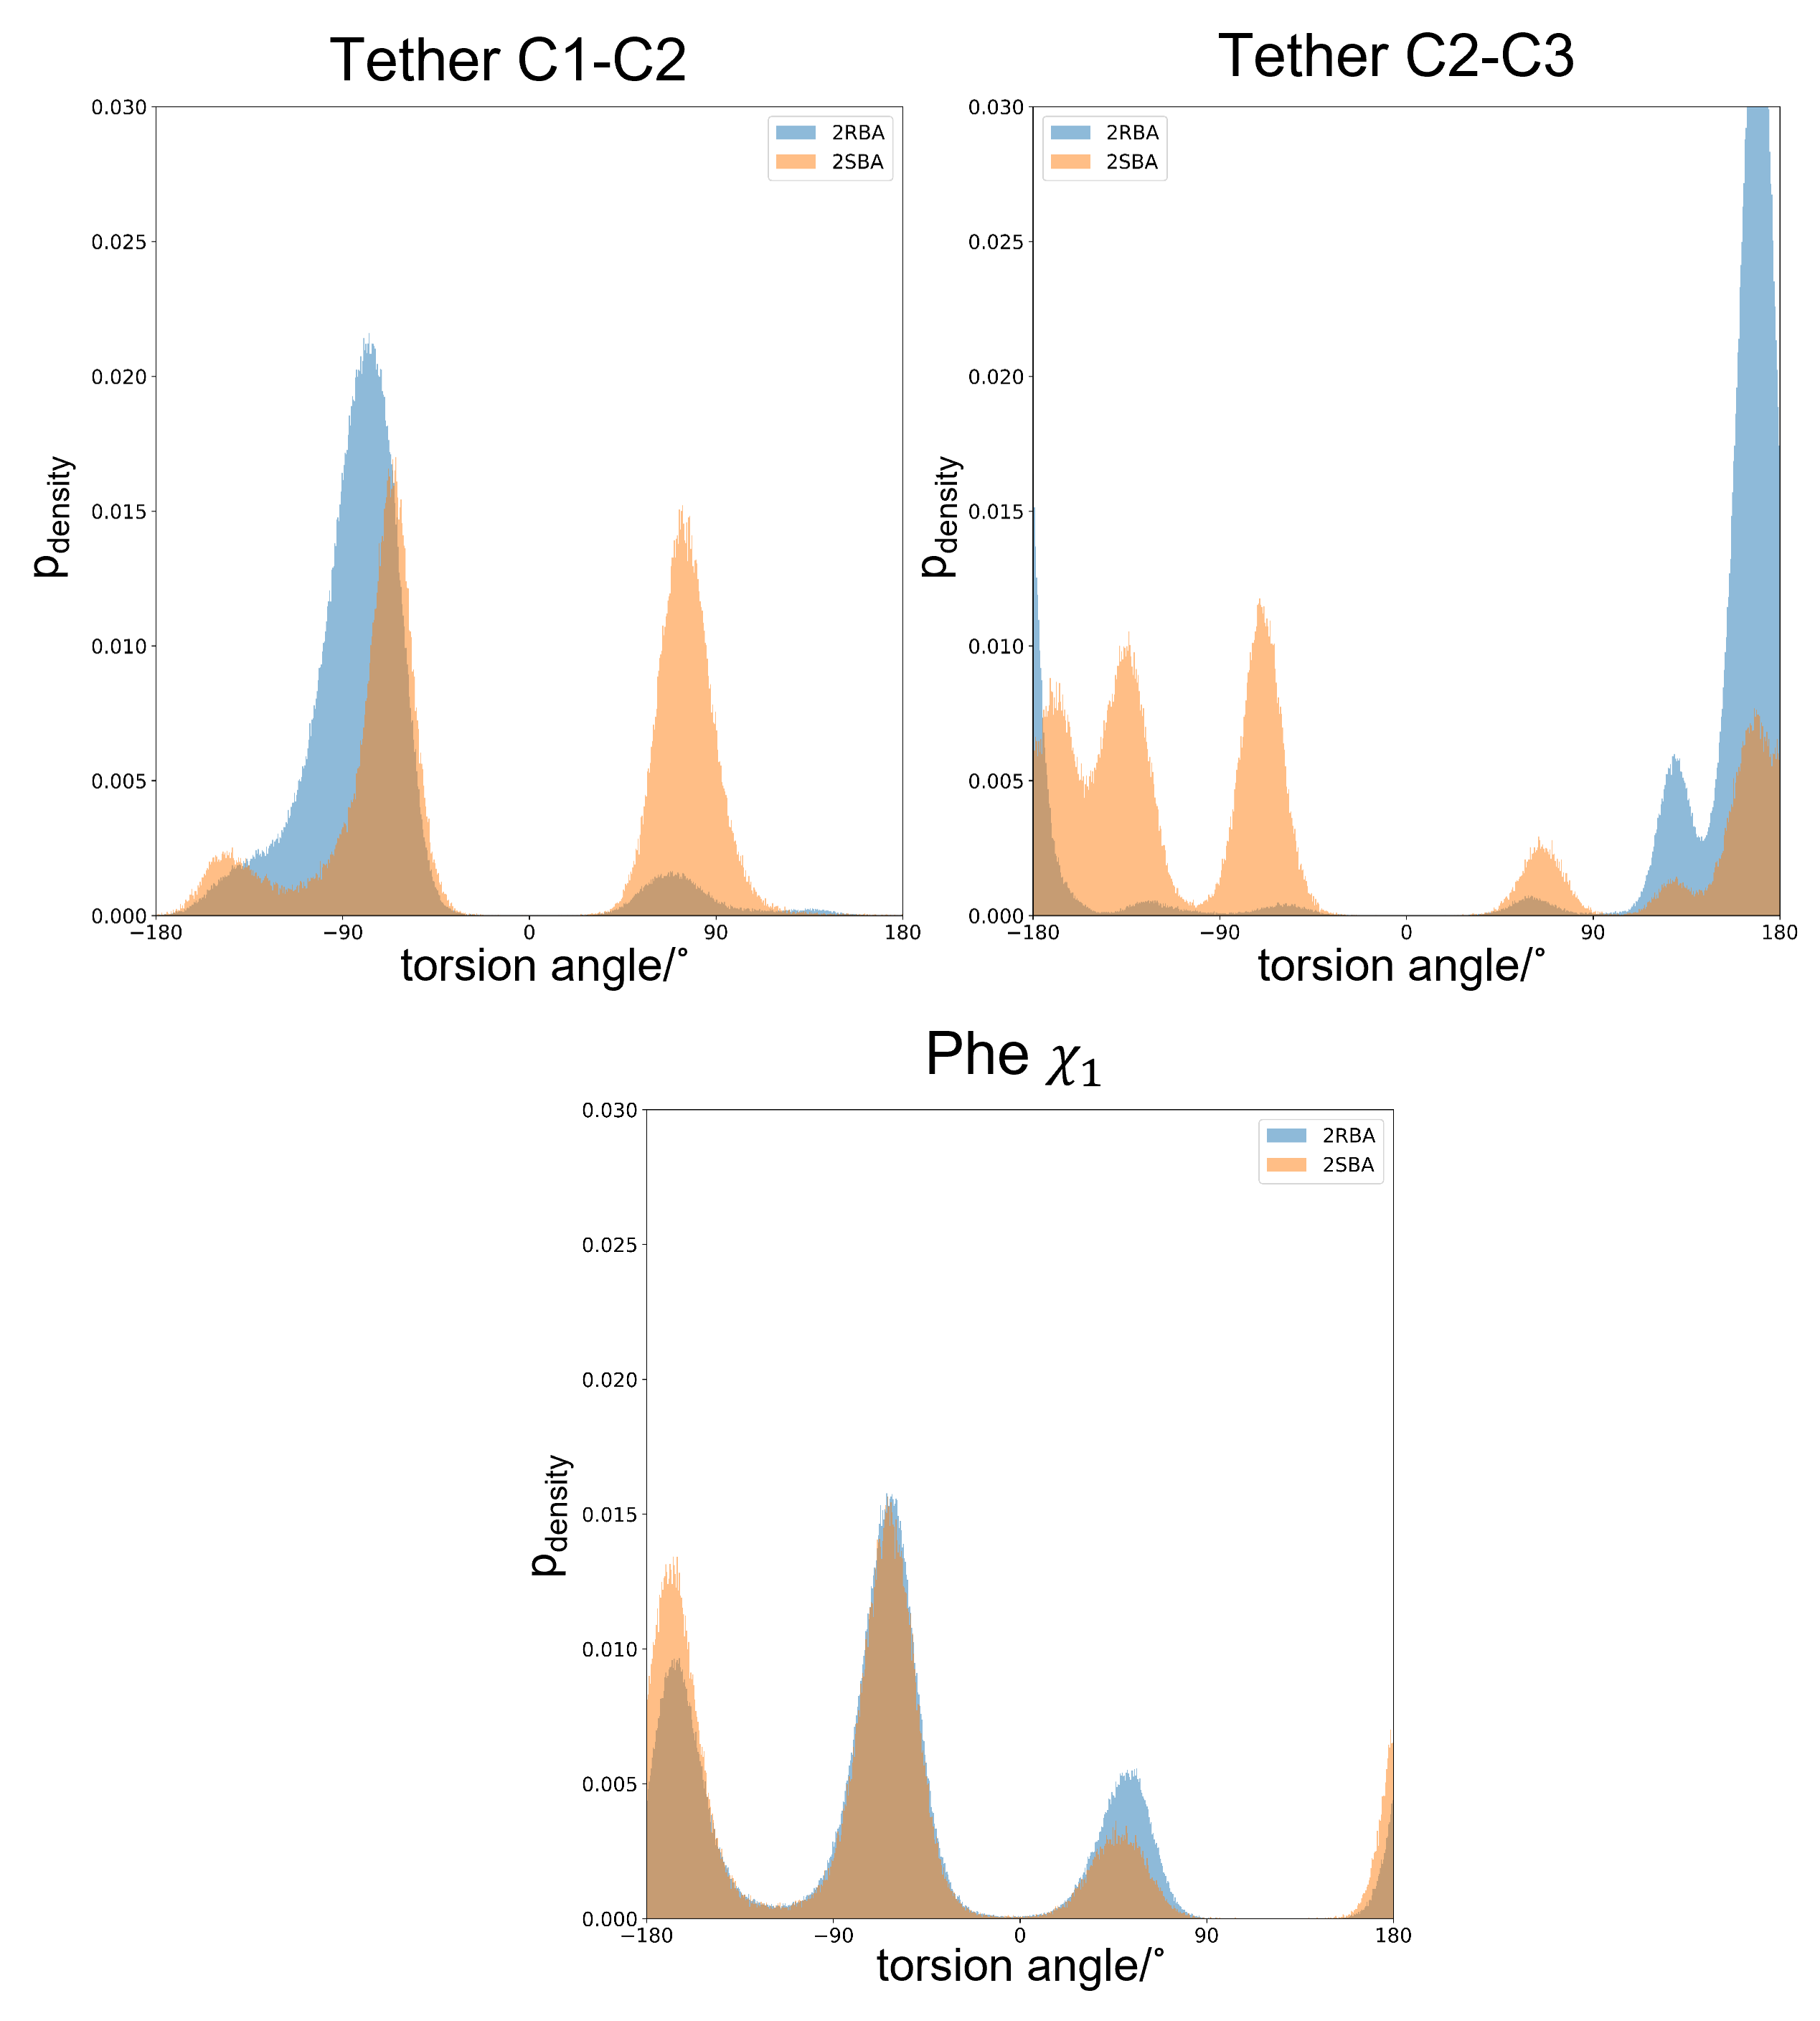
\includegraphics[width=\textwidth]{7_chapter_5/fig/results/dihedral_dist_2RS.png}
    \caption{Torsional-angle distributions of the tether in Nleu-2R (blue) and Nleu-2S (orange) in chloroform. Analysis was restricted to the clusters with the trans-peptoid bond. The distribution density is plotted as a function of the torsional angle, with a bin size of $0.5~\text{deg}$.}
    \label{fig: SITorsion2RS}
\end{figure}


\FloatBarrier
%-------------------------------------------

\begin{table}[h!]
    \centering
    \caption{Percentage of sampled conformations with zero, one, or two hydrogen bonds for Nleu-5R, Nleu-5S, Nleu-2R, and Nleu-2S in water. Analysis was restricted to the clusters with the trans-peptoid bond.}
    \label{tab: hbondsratiowater}
    \begin{adjustbox}{max width=\textwidth}
    \begin{tabular}{lccc}
    Number of hydrogen bonds [\%] &	0 &	1 &	2 \\
    \hline
    Nleu-5R  &	87	& 12	& 1 \\
    Nleu-5S  &	74	& 26	& 0  \\
    Nleu-2R  &	78	& 22	& 0 \\
    Nleu-2S  &	76	& 24	& 0 \\
    \hline
    \end{tabular}
    \end{adjustbox}
\end{table}

The analysis of the hydrogen-bonding patterns in water showed a significant decrease for the intramolecular H-bond populations, as they competed with the intermolecular H-bonds to the water. Specifically, Nleu-5R has a higher percentage (about $10\%$) of conformers with no H-bonds compared to Nleu-2R, Nleu-2S, and Nleu-5S (Table \ref{tab: hbondsratiowater}). The conformations containing two intramolecular H-bonds nearly vanished.
The positions of the intramolecular H-bonds are mainly focused on the Nleu-O and tether-NH position (Table \ref{tab: SIhbondRatiosWater}).
Nevertheless, it could be observed that the Ala-O and tether-NH, which was unique to Nleu-5S in the apolar environment, is again most present in water for Nleu-5S in contrast to the other possible intramolecular H-bonds. 
In general, however, no significant differences between the peptides could be observed in water.

\begin{table}[h!]
\centering
\caption{Hydrogen-bond occurrence in percentage for the sampled conformations in
water for Nleu-5R, Nleu-5S, Nleu-2R, and Nleu-2S. The analysis was restricted to the clusters with the trans-peptoid bond.}
\label{tab: SIhbondRatiosWater}
  \begin{adjustbox}{max width=\textwidth}
  \begin{tabular}{lcccc}
Hydrogen bond {[}\%{]} & Nleu-2R      & Nleu-2S      & Nleu-5R      & Nleu-5S      \\
\hline
Nleu-O tether-NH       & 14.5       & 18.3       &  12           & 9.75        \\
Ala-O tether-NH        & 5.5        & 3.6        & \textless{}1  & 15.25 \\
Phe-O Ala-NH           & \textless{}1 & \textless{}1 & \textless{}1  & 1 \\
Ala-O Phe-NH           & 2            & 1            & \textless{}1  & \textless{}1 \\
    \hline
\end{tabular}%
\end{adjustbox}
\end{table}


\FloatBarrier
%-------------------------------------------

The findings, taken together, suggest that the permeability cliff observed between Nleu-5R and Nleu-5S is related to their propensity for conformations with a maximized number of intramolecular H-bonds in the apolar environment. Their ability to adopt such conformations is in turn affected by the stereochemistry of the methyl group at position $5$ in the tether as it determines the preferred torsional angles of the tether.



\clearpage
\newpage

%================================================================================
\section{Conclusion}
%================================================================================

Combining the permeability data generated by our collaborators, NMR measurements, and MD simulations allowed us to draw some conclusions on how the structural differences between the selected macrocycles influence their membrane permeability. 
The pair of Nleu-2R/S did not show a significant change in permeability depending on the stereocenter change. In contrast, the second pair Nleu-5R/S showed a significant effect on permeability behavior. Nleu-5R is the most permeable compound from the compound collection synthesized by our collaborators, while Nleu-5S is with its low permeability the exception among the Nleu compounds. 
In the MD simulations, we observed different H-bond patterns for Nleu-5R and Nleu-5S in the chloroform. While Nleu-5R frequently adopted a conformation with the maximum number of two H-bonds (optimal shielding of the polar groups), such a conformation was rare for Nleu-5S. A detailed analysis of the torsional angle preferences highlighted the underlying steric effects.

In contrast to other studies, we could not retrieve a correlation between the 3D-PSA and the PAMPA permeability for the four selected macrocycles. The backbone cycle of the peptides is relatively small, thus minor structural changes affecting the geometry of the intramolecular H-bonds are likely not reflected appropriately in the 3D-PSA calculation.
In summary, we studied the relationship between small structural changes and the resulting permeability behavior for four semipeptidic macrocycles. The location and especially the stereochemistry of the methyl group played an important role in the intramolecular hydrogen-bonding pattern, impacting the passive membrane permeability of the compounds.


\clearpage
\pagebreak

%================================================================================
%\section{Appendix}
%================================================================================
\begin{ethappendix}
%================================================================================
%\appsection[CBTI and Quadrature]{quad}{Relationship between CBTI and Quadrature Integration}
%================================================================================

\end{ethappendix}
\clearpage
\pagebreak

%% %================================================================================
%% \begin{thebibliography}{74}
%% \input{\path/inc/paper.lrs}
%% \end{thebibliography}
%% %================================================================================

\end{document}
